\documentclass[a4paper,12pt,oneside,final]{extarticle}
\usepackage[top=2cm, bottom=2cm, left=3cm, right=1cm]{geometry}
\usepackage{scrextend}

\usepackage{fontspec}  
\usepackage{polyglossia}

\usepackage{tempora}
\setmainfont{tempora}
\setmainlanguage{russian} 
\setotherlanguages{english,ukrainian}


\frenchspacing

% Lists
\usepackage{enumitem}
\renewcommand\labelitemi{--}
\renewcommand\labelenumi{\arabic*}
\setlist[description]{noitemsep,style=multiline,leftmargin=2.5cm}
\setlist[itemize]{noitemsep}
\setlist[enumerate]{noitemsep}

\usepackage{titlesec}
\newcommand{\sectionbreak}{\clearpage}

\usepackage{hyperref} % make refs clickable
\usepackage{float}
\usepackage{pgfplots}
\usepackage{graphicx}
\usepackage{multirow}
\usepackage{amssymb,amsfonts,amsmath,amsthm}
\usepackage{csquotes}
\usepackage{xstring}
\usepackage{tabularx}

\numberwithin{equation}{section}

\usepackage{listings}
\lstset{basicstyle=\footnotesize\ttfamily,breaklines=true}
\lstset{language=Matlab}

\makeatletter
\def\maxwidth#1{\ifdim\Gin@nat@width>#1 #1\else\Gin@nat@width\fi}
\makeatother

\begin{document}
\title{Основы управление развитием организации}
\maketitle
\tableofcontents

%
% section 1
%
\section{Модуль I}
\subsection{Понятие и сущность управления}
Управление --- это эффективное использование и координация таких ресурсов, как капитал, здания, материалы и труд для достижения заданных целей с максимальной эффективностью.

\begin{figure}[h]
	\centering
	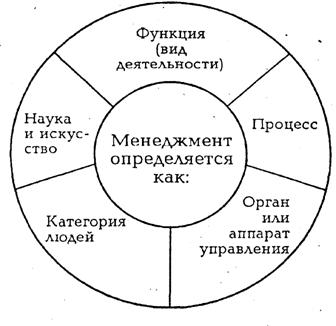
\includegraphics[width=\maxwidth{\textwidth}]{management-figures/management}
	\caption{Подходы к определению сущности и роли менеджмента}
\end{figure}

Система менеджмента включает следующие компоненты:
\begin{itemize}
	\item механизм управления:
	\begin{itemize}
		\item общие принципы управления;
		\item функции управления; 
		\item цели;
		\item методы управления; 
	\end{itemize}
	\item структуру управления:
	\begin{itemize}
		\item общую структуру управления;
		\item конкретную систему органов управления;
		\item кадры управления;
		\item технические средства управления.
	\end{itemize}
	\item процесс управления \textit{(включает содержательную и организационную его характеристики, организацию принятия и реализации решений, технологию и процедуры управления, организацию деятельности работников управления)};
	\item механизм развития системы управления.
\end{itemize}

\subsection{Управление и менеджеры}
Требования к профессиональной компетенции менеджеров можно условно разделить на две группы:
\begin{enumerate}
	\item \textbf{Первые} представляют знания и умение выполнять профессиональную работу в такой специальной области как менеджмент. 
	Они включают:
	\begin{enumerate}
		\item Умение обосновывать и принимать решения в ситуациях,  для которых характерны высокая динамичность и неопределенность.
		\item Высокую информированность по вопросам развития отрасли, в которой работает организация \textit{(состояние исследований, техники, технологии, конкуренции и т.д.)}.
		\item Знакомство с опытом менеджмента в других организациях и разных отраслях.
		\item Способность управлять ресурсами, планировать и прогнозировать работу организации, владение способами повышения эффективности управления.
		\item Умение использовать современную информационную технологию, средства коммуникации и связи.
	\end{enumerate}
	\item \textbf{Вторая} группа связана со способностью работать с людьми и управлять самим собой:
	\begin{enumerate}
		\item Высокое чувство долга и преданность делу.
		\item Честность в отношениях с людьми и доверие к партнерам.
		\item Умение четко выражать свои мысли и убеждать.
		\item Уважительное и заботливое отношение к людям вне зависимости от их положения в иерархии организации.
		\item Способность быстро восстанавливать свои физические и душевные силы и критически оценивать собственную деятельность.
	\end{enumerate}
\end{enumerate}

Повышение результативности менеджмента достигается разделением труда, выделяют следующие виды разделения труда менеджеров в организации:
\begin{itemize}
	\item \textbf{Функциональное} разделение труда основывается на формировании групп работников управления, выполняющих одинаковые функции менеджмента \textit{(планирование, контроль, организация)}.
	\item \textbf{Структурное} разделение труда \textit{(вертикальное и горизонтальное)} строится исходя из таких характеристик управляемого объекта как организационная структура, масштабы сферы деятельности, отраслевая или территориальная специфика. 
	Такое разделение труда специфично для каждой организации.
	\item \textbf{Технологическое} и \textbf{профессионально-квалификационное} труда учитывает виды и сложность выполняемых работ. 
\end{itemize}

\subsection{Развитие теории и практики управления}
История развития менеджмента насчитывает несколько тысячелетий.

\textbf{Первая} управленческая революция --- религиозно-коммерческая.

\textbf{Вторая} --- 1760 г. до н.э. связывается с деятельностью царя Хаммурапи, издавшего свод законов управления государством для регулирования всего многообразия общественных отношений между различными социальными группами населения.

\textbf{Третья} --- 605-682 г. до н.э. направлена на соединение государственных методов управления  с контролем за деятельностью в сфере производства и строительства.

\textbf{Четвертая} --- 17-18 в н.э. связана с зарождением капитализма и началом индустриального прогресса европейской цивилизации. 
Главное революционное преобразование в области менеджмента --- это отделение его от собственности и зарождение профессионального менеджмента.

\textbf{Пятая} --- конец 19 - начало 20 века --- бюрократическая. 
Теоретическая платформа преобразования в области управления --- концепция бюрократии, позволившая  сформировать крупные иерархические структуры менеджмента, осуществить разделение труда, ввести нормы и стандарты, установить должностные обязанности и ответственность менеджеров. 

Развитие менеджмента в основном эволюционный процесс.

К концу 19 - началу 20 веков  появились первые работы, в которых была сделана попытка научного обобщения накопленного опыта  и формирования основ науки менеджмента:
\begin{enumerate}
	\item Подход с позиции выделения различных школ.
	\begin{itemize}
		\item \textbf{Школа научного управления} \\
		Концепция этой школы --- переломный этап, благодаря которому управление стало признаваться как самостоятельная область научных исследований. 
		Первой фазой методологии научного управления были анализ содержания работы и определение ее основных компонентов.
		\item \textbf{Классическая школа в управлении} \\
		Цель этой школы --- создание универсальных принципов управления, которые затрагивали два основных аспекта:
		\begin{itemize}
			\item разработка рациональной системы управления организацией; 
			\item построение структуры организации и управления работниками.
		\end{itemize}
		\item \textbf{Школа человеческих отношений} \\
		Мотивы поступков людей в основном зависят от потребностей, которые могут быть лишь частично и косвенно удовлетворены с помощью денег. 
		Если руководство проявляет большую заботу о своих работниках, то возрастает уровень удовлетворенности работников, что ведет к увеличению производительности.
		\item \textbf{Школа поведенческих наук} \\\
		Сосредоточение на методах налаживания межличностных отношений. 
		Главный постулат --- правильное применение науки о поведении всегда будет способствовать повышению эффективности как отдельного работника, так и организации в целом.
		\item \textbf{Школа науки управления или количественный подход} \\ 
		Общее название --- исследование операций. 
		Сущность --- применения методов научного исследования к операционным проблемам организации.
	\end{itemize}
	\item \textbf{Процессный подход}.
	\item \textbf{Системный подход}.
	\item \textbf{Ситуационный подход}.
\end{enumerate}

\subsection{Современная система взглядов на управление}
Принципиальные положения современной системы взглядов на менеджмент:
\begin{enumerate}
	\item Отказ от управленческого рационализма классической школы менеджмента, выражающегося в убеждении, что успех организации определяется воздействием  управления на внутренние факторы организации. 
	Вместо этого на первое место выдвигается проблема гибкости и адаптивности к постоянным изменениям внешней среды.
	\item Использование в управлении теории систем. 
	Организация рассматривается в единстве ее составных частей, которые неразрывно  связаны с внешним миром.
	\item Использование ситуационного подхода к управлению. 
	Признается важность специфических приемов, с помощью которых выделяются факторы, воздействуя на которые можно эффективно достичь цели.
	\item Признание социальной ответственности менеджмента как перед обществом в целом, так и перед отдельными людьми, работающими в организации. 
\end{enumerate}

\subsection{Определение <<организационная система>>. Организационные системы как системы междисциплинарной природы}
Организация в зависимости от контекста:
\begin{description}
\item[Свойства] Внутренняя упорядоченность, согласованность взаимодействия более или менее дифференцируемых и автономных частей целого обусловленного его строением.
\item[Процесс] Совокупность процессов или действий, ведущих к образованию и совершенствованию взаимосвязей между частями целого.
\item[Орг. система] Объединения людей совместно реализующих некоторую программу или цель, действующих на основе определенных процедур и правил.
\end{description}

При рассмотрении организации как объектов управления большую роль играют и назначения, размеры, строение и другие характеристики. 
Организация может быть описана с помощью разных параметров: целевое назначение, правовая и нормативная основа, ресурсы, процессы, структура, разделение труда.

Классификация организаций:
\begin{enumerate}
	\item \textbf{По формализации}:
	\begin{itemize}
		\item формальные организации (имеют четко поставленные цели, формализованные правила, структуру и связи; в эту группу входят все организации бизнеса, государственные и международные институты и органы);
		\item неформальные организации (работающие без четко определенных целей, правил и структур; сюда относят все институты семьи, дружбы, неформальных отношений между людьми).
	\end{itemize}
	\item \textbf{По формам собственности}:
	\begin{itemize}
		\item частные;
		\item государственные;
		\item муниципальные и т.д..
	\end{itemize}
	\item \textbf{По отношению к прибыли}:
	\begin{itemize}
		\item коммерческие (основная цель --- получение прибыли);
		\item некоммерческие (не стремятся извлекать или распределять полученную прибыль между участниками, но могут осуществлять предпринимательскую деятельность, когда это служит достижению целей, ради которых они созданы, и соответствуют этим целям).
	\end{itemize}
	\item \textbf{По размерам}:
	\begin{itemize}
		\item крупные;
		\item средние;
		\item малые.
	\end{itemize}
	\item \textbf{По участию в различных секторах производства} организации делят на четыре типа, в каждый из которых входит несколько отраслей, однородных по своему месту в технологическом цикле:
	\begin{itemize}
		\item отрасли первичного цикла, занимающиеся добычей сырья (включают организации и предприятия сельского, лесного и рыбного хозяйств, угольной промышленности);
		\item отрасли вторичного цикла, в который входят организации и п/п обрабатывающей промышленности (машиностроение, металлообработки и т.д.);
		\item отрасли третичного цикла, в который входят организации и п/п услуги которых необходимы для нормальной трудоспособности отраслей первых двух секторов (банки, отраслевые компании, образовательные учреждения, турагенства, внешняя торговля и др.)
		\item к четвертому сектору относят все организации и институты, которые занимаются информационными технологиями.
	\end{itemize}
\end{enumerate}

\subsection{Внутренняя и внешняя среда организационной системы}
Внутренняя среда организационной системы --- это ее организационное строение и ситуационные факторы внутри нее (внутренние переменные).
К основным переменным относятся: 
\begin{itemize}
	\item структура;
	\item цели;
	\item задачи;
	\item технологии; 
	\item люди.
\end{itemize}

Внешняя среда организации --- это силы внешние по отношению к организации, которые действуют на ее результативность. 
Факторы, оказывающие немедленное воздействие или влияние на организацию --- это \textbf{среда прямого воздействия}, а все другие --- \textbf{косвенного}.

Выделяют 4 основных свойства внешней среды: 
\begin{itemize}
	\item взаимосвязанность факторов внешней среды \textit{(уровень силы, с которой изменение одного фактора воздействует на другие)}; 
	\item сложность внешней среды \textit{(количество факторов и уровень вариативности)}; 
	\item подвижность среды \textit{(скорость, с которой могут меняться факторы)}; 
	\item неопределенность среды \textit{(является функцией количества информации, которой располагает организация по поводу конкретного факторы, а также функция уверенности в этой информации)}. 
\end{itemize}

\subsection{Задачи управления организационными системами}
Управление ОС, понимаемое как воздействие на управляемую систему с целью обеспечения требуемого ее поведения, может затрагивать каждый из следующих шести параметров ее модели:
\begin{enumerate}
	\item Управление составом.
	\item Управление структурой.
	\item Институциональное управление \textit{(управление ограничениями и нормами деятельности)}.
	\item Мотивационное управление \textit{(управление предпочте­ниями и интересами)}.
	\item Информационное управление \textit{(управление информацией, ко­торой обладают участники ОС на момент принятия решений)}.
	\item Управление порядком функционирования \textit{(управление последовательностью получения информации и выбора стратегий участниками ОС)}.
\end{enumerate}
\begin{figure}[h]
	\centering
	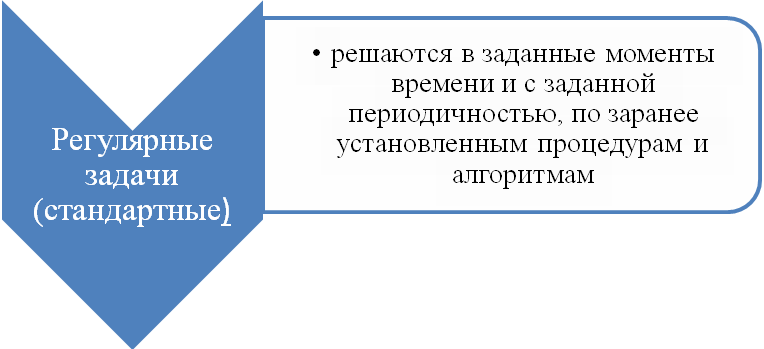
\includegraphics[width=\maxwidth{\textwidth}]{management-figures/non_regular_organization_management_tasks}
	\caption{Нерегулярные задачи}
\end{figure}
\begin{figure}[h]
	\centering
	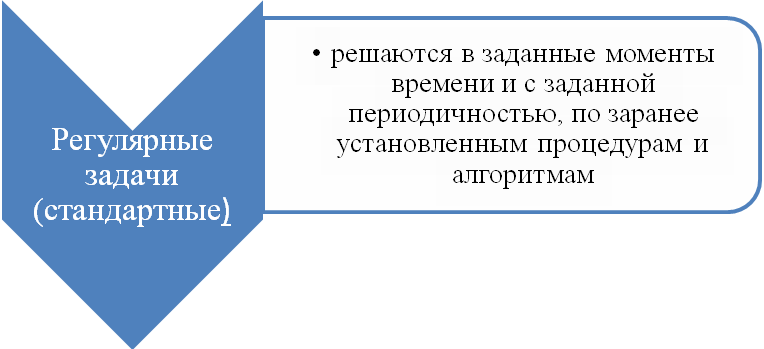
\includegraphics[width=\maxwidth{\textwidth}]{management-figures/regular_organization_management_tasks}
	\caption{Регулярные задачи}
\end{figure}
Задача принятия решения становится проблемой, когда для постановки задачи и ее решения не может быть сразу определен подходящий аппарат формализации --- требуется разработка специальных подходов, приемов и методов. 
При этом процесс постановки задачи часто требует участия специалистов различных областей знаний. В таких случаях возникает необходимость:
\begin{itemize}
	\item определить область проблемы принятия решения \textit{(границы системы)};
	\item выявить факторы, влияющие на ее решение \textit{(входы системы и внутренние факторы, влияющие на целевой выход)};
	\item подобрать приемы и методы, которые позволяют сформулировать или поставить задачу таким образом, чтобы решение было принято.
\end{itemize}

\subsection{Понятие принципа и роль в управлении организационной системой}
Принципы управления --- базовые постулаты, которые определяют строение и работу системы управления организации. 
Сегодня в сфере управления применяются следующие принципы руководства: 
\begin{itemize}
	\item гармоничного \textbf{совмещения централизации и децентрализации}, что предусматривает полноправную передачу прав по ходу принятия решений. 
	Здесь происходит сочетание принципа лидерской самодостаточности с умелой командной работой для достижения результата; 
	\item \textbf{научного подтверждения}, предполагающего предвидение намеченных социально-экономических реформ компании благодаря привлечению разработанных систем, методик и подходов; 
	\item \textbf{планирования}, определяющего основополагающие действия в функционировании и развитии организации;
	\item \textbf{комбинирования прав, обязательств и поручительств} --- это предполагает права и обязанности каждого подчиненного за его сферу деятельности; 
	\item \textbf{самостоятельности}, то есть персональной независимости индивидов, выполняющих управленческую деятельность в законных рамках; 
	\item \textbf{иерархии и отклика} --- задачи для подчиненных ставятся руководством; 
	\item \textbf{стимулирования} --- результативность обеспечивается благодаря наказаниям, а также поощрениям;
	\item \textbf{демократичности}, предполагающей вклад в функционирование фирмы каждого работника.
\end{itemize}
\begin{figure}[h]
	\centering
	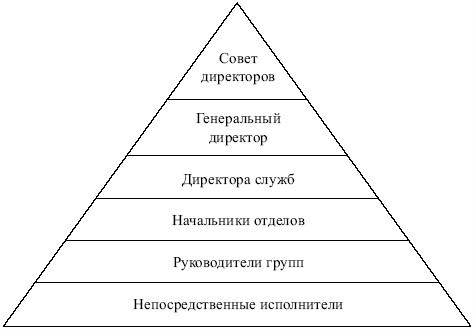
\includegraphics[width=\maxwidth{\textwidth}]{management-figures/roles_in_organized_systems}
	\caption{Уровни управления \textit{(роли проекта)}}
\end{figure}

\subsection{Содержание основных принципов управления}
При всех условиях управление персоналом осуществляется на основе следующих традиционно утвердившихся в организациях принципов: 
\begin{itemize}
	\item научность, централизм, плановость, первое лицо, единство распорядительства; 
	\item отбор, подбор и расстановка кадров; сочетание единоначалия и коллегиальности, централизации идей рализации; 
	\item линейное, функциональное и целевое управление, контроль исполнения решений и др. 
	Ряд американских и японских корпораций широко используют следующие принципы управления персоналом: пожизненный найм, контроль исполнения заданий, основанный на доверии; 
	\item сочетание такого контроля с корпоративной культурой; 
	\item консенсуальное принятие решений, обязательное одобрение принимаемых решений большинством работников.
\end{itemize}

Обратимся к основным принципам управления персоналом, выделенным В. И. Кноррингом:
\begin{enumerate}
	\item \textbf{Принцип цели}. \\ 
	Каждое действие должно иметь ясную и определенную цель;
	\item \textbf{Принцип правовой защищенности управленческого решения}. \\ 
	Знание действующего законодательства и принятие управленческих решений только с учетом соответствия этих решений действующим правовым актам;
	\item \textbf{Принцип оптимизации управления} --- повышение эффективности управляемой системы;
	\item \textbf{Принцип соблюдения нормы управляемости}. \\ 
	Любое управленческое решение должно соответствовать возможностям упраляемой системы. 
	Управляющее воздействие не должно быть столь экстремальным, чтобы вывести объект управления из зоны управляемости (если только такая задача не стоит специально). 
	Подавляющее большинство управляющих воздействий должно соответствовать нормам управляемости объекта воздействия;
	\item \textbf{принцип соответствия}. \\
	Порученная работа должна соответствовать функциональным обязанностям \textit{(установленной области компетенции)}, интеллектуальным и физическим возможностям исполнителя.
	\item \textbf{Принцип автоматического замещения отсутствующего}. \\ 
	Замещение отсутствующих должно решаться автоматически на основе действующих служебных должностных инструкций и регулироваться формально. 
	Следствие этого принципа --- важность служебных должностных инструкций, документов, направленных на выполнение своего долга.
	\item \textbf{Принцип первого руководителя} \\ 
	При организации выполнения важного производственного задания контроль за ходом работ должен быть оставлен за первым руководителем предприятия, так как только первое лицо имеет право и возможность решать или поручать решение любого вопроса, возникающего при внедрении этого мероприятия.
	\item \textbf{Принцип одноразового ввода информации}. \\ 
	Информация вводится в базу знаний только один раз, а доступ к ней обеспечивается для многих пользователей. 
	Следование этому принципу позволяет объединять используемую информацию, обеспечивать единство информационной базы принимаемых решений и избегать дублирования.
	\item \textbf{Принцип повышения квалификации}. \\
	Персонал только в том случае будет соответствовать непрерывно меняющимся и усложняющимся требованиям рынка, когда будет постоянно повышать свою квалификацию, осваивать новые технологии и т.п.
\end{enumerate}

\subsection{Цели организационных систем и их классификация}
Одним из важнейших критериев является период времени, на который устанавливаются цели. 
По этому критерию выделяют три группы целей:
\begin{enumerate}
	\item \textbf{Стратегические}, устанавливаемые на длительный период (его продолжительность колеблется в зависимости от состояния и ус­тойчивости развития экономики от трех до 5-10 лет); важным моментом разработки стратегических целей является ориентация на потребности клиентов, которая нередко предопределяет успех организации в острой конкурентной борьбе;
	\item \textbf{Тактические}, являющиеся логическим развертыванием стра­тегических целей и устанавливаемые на более короткие периоды (от одного до 3-5 лет для условий стабильного развития); они характеризуются конкретизацией плановых заданий, которые чаще всего получают количественное измерение;
	\item \textbf{Оперативные}, представляющие собой детализацию стратегических и тактических целей до уровня задач, которые должны решать конкретные исполнители в своей повседневной работе в пределах года, полугодия, квартала, месяца, рабочего дня.
\end{enumerate}

Группировка целей по содержанию построена на многообразии интересов организации. 
Так, в коммерческих организациях превалируют экономические интересы, т.е. стремление получить прибыль, обеспечить дивиденды акционерам и оплату труда работающим и т.п. 
В соответствии с этим формируется состав экономиче­ских целей организации, в котором ключевая роль отводится финансовым показателям. 
Наряду с этим любая организация ставит цели, отражающие социальные интересы людей (подготовка и обучение персонала, повышение квалификации и продвижение, взаимоотношения в коллективе, условия и содержание труда и т.д.), планируемые организационные изменения (в структуре самой организации и ее системы управления), преобразования в области научных исследований и технологий и т.п.

По значимости цели подразделяются на: особо приоритетные, с достижением которых связано получение главного результата развития организации; приоритетные, необходимые для успеха и требующие внимания руководства; остальные, также важные, но несрочные цели, нуждающиеся в постоянном контроле.
Группировка целей по критерию повторяемости имеет значение для разработки способов их достижения. 
Для постоянных и периоди­чески повторяющихся целей, как правило, в организации имеются методики, а также ресурсы и люди, способные их использовать.

\subsection{Понятие об управленческом цикле}
Управленческий цикл — это завершенная последовательность повторяющихся действий, направленных на достижение поставленных целей.

Управленческий цикл начинается с уяснения задачи или проблемы и заканчивается достижением определенного результата. 
После этого цикл управления повторяется. Частота его повторения определяется конкретным типом и природой управляемой системы. 
В социальных системах этот цикл повторяется непрерывно. 
Конечная цель управления системой может достигаться одним или несколькими циклами управления.

Циклическая реализация процессов позволяет устанавливать и фиксировать характерные черты, общие зависимости, единые закономерности процессов и обеспечивать на этой основе их рациональную процессуализацию и предвидение.
В характеристиках управленческого процесса используются также более узкие понятия:

\begin{itemize}
	\item период, имеющий хронологическое значение;
	\item действия и операции --- целостные и четко обособленные части процесса;
	\item процедура --- определенная регламентированная последовательность осуществления процесса.
\end{itemize}

Основные этапы управленческого цикла:
\begin{enumerate}
	\item Сбор и обработка информации, анализ, уяснение и оценка обстановки — диагноз.
	\item Научно обоснованное предсказание наиболее вероятного состояния, тенденций и особенностей развития объекта управления на период упреждения на основе выявления и правильной оценки устойчивых связей и зависимостей между его прошлым, настоящим и будущим — прогноз.
	\item Выработка и принятие управленческого решения.
	\item Разработка системы мер, направленных на достижение поставленной цели — планирование.
	\item Своевременное доведение до исполнителей поставленных задач, правильный подбор и расстановка сил, мобилизация исполнителей на выполнение принятого решения — организация.
	\item Активация деятельности исполнителей — мотивация и стимулирование.
	\item Получение, обработка, анализ и систематизация сведений о ходе реализации заданий, проверка того, насколько организация дела и результаты исполнения соответствуют принятым решениям, — учет и контроль.
\end{enumerate}

Общий для 4-х последних этапов — обеспечение пропорционального и непрерывного функционирования всей системы управления путем установления текущих оптимальных связей между отдельными исполнителями — регулирование.

\subsection{Характеристика функций управления}
Функции управления --- это определенные виды управленческой деятельности, выделившиеся в процессе специализации управленческого труда.

Функции управления носят объективный характер, поэтому их применение должно быть основано на познании принципов управления и учете конкретной обстановки. 
Они универсальны, т.к. характеризуют любой процесс управления.

Для выполнения функций управления должны быть созданы управленческие должности и организационная структура управления, для того чтобы установить, кто конкретно выполняет функции и каким образом управленческие работники взаимодействуют между собой.

Функции управления делятся на 2 группы: общие (основные); специальные.
\textbf{Общие функции управления} осуществляются в каждой производственной системе и на каждом уровне управления. 

Весь процесс управления представляется как цепь последовательных, циклически повторяющихся общих функций: планирование, организация, мотивация и контроль.

\textbf{Функция планирования} --- представляет собой управленческую деятельность, которая предусматривает выработку целей и задач управления организацией, а так же определение путей реализации планов для достижения поставленных целей.

\textbf{Цель планирования} --- это определение будущего состояния, тенденций и перспектив развития объекта управления.
Планирование устанавливает связи между существующим положением дел на предприятии и тем, которое должно быть достигнуто в будущем, что даст возможность реализовать представившиеся возможности и свести к минимуму будущие риски. Результатом выполнения функции планированияявляется --- план.

\textbf{Функция организации} --- представляет собой управленческую деятельность, которая заключается в установлении взаимоотношений между всеми подразделениями,рабочими местами и работниками и координации их действий. 
Цель функции организации --- формирование структуры субъекта и объекта управления, а также их взаимосвязей. 
Функция организации, по сути, состоит в формировании управляющей и управляемой подсистем субъекта хозяйствования, а также в налаживании связей между этими подсистемами. 

Содержание функции организации в менеджменте раскрывается через такие понятия как: «департаментализация», «делегирование», «диапазон контроля», «централизации и децентрализации управления», регламентация. 
Результатом выполнения функции организации является создание организационной структуры управления предприятием и организационного процесса управления.

\textbf{Мотивация} – процесс побуждения работников и себя к активной трудовой деятельности для достижения личностных целей и целей предприятия, т.е. создание у работников внутренних (психологических) побуждений к труду. 
Главными здесь являются: заинтересованность в труде, потребность в трудовой активности, удовлетворенность от трудовой деятельности.
Цель мотивации – побудить сотрудников к достижению целей организации, путем обеспечения их заинтересованности в результатах собственного и совместного труда.
Функция мотивации оказывает влияние на коллектив предприятия или его подразделения в форме побудительных мотивов к эффективному труду, общественного воздействия, коллективных и индивидуальных поощрительных мер и т.д. 

\textbf{Контроль} как функция управления призван обеспечить достижение целей организации путем систематического представления информации о действительном состоянии дела по выполнению плановых заданий, решений, нормативно установленных задач и предписаний, путем анализа этой информации и проведения соответствующих корректировок. 
Цель контроля заключается в том, чтобы предупреждать возникновение кризисных ситуаций. 
Контроль включает учет, анализ и регулирование. 
По итогам учета менеджер должен получить объективную информацию о реальном состоянии объекта управления.

\subsection{Понятие коммуникаций и их роль в системе управления}
Эффективность работы менеджера зависит как от его умения работать с людьми, так и от того, как он работает с информацией Основным требованием для принятия эффективного объективного решения или даже раз нимание масштабов проблемы является наличие точной информации.

\textbf{Коммуникация} --- процесс обмена информацией и смысловым значением между двумя или более людьми (то есть передача информации)

Прочность и качество отношений между людьми (друзьями, членами семьи или коллегами) является отражением того, насколько четкими и честными являются их межличностные отношения

Поскольку организация --- структурированный тип отношений между людьми, она в значительной степени зависит от качества коммуникаций и обеспечения эффективного функционирования.
Если коммуникации не будут эффективными, люди не смогут договорить ся об общей цели, что составляет предпосылку функционирования организации.

Информация в процессе коммуникации передается не только с целью принятия разумных решений, но и для того, чтобы они могли выполняться.
Конечно, если руководство предоставляет подчиненным информацию о обоснованием ния своих решений, это значительно увеличивает шансы их успешного выполнения до тех пор, пока работники не поймут, какое вознаграждение им предложит организация за качественно выполненную работу, они не могут на нее хорошо работать.

Коммуникация также важна и для функции контроля.

Цели коммуникации:
\begin{itemize}
	\item Организовывать информационный обмен между субъектом и объектом управления.
	\item Наладить процесс эмоционального и интеллектуального обмена управленческой информацией.
	\item Установить взаимосвязь между людьми в организации.
	\item Сформулировать общие взгляды на внутреннюю среду организации.
	\item Организовать совместную работу коллективов с целью выполнения задач организации.
\end{itemize}
Значение коммуникации в организации:
\begin{itemize}
	\item Коммуникация --- основное условие существования и развития организации.
	\item Коммуникация осуществляет взаимодействие с внешней средой, определяя уровень и качество принятия управленческих решений.
	\item Коммуникации характеризуют состояния внутренней среды организации путем обеспечения функционирования и взаимодействия людей, структуры, целей, технологии и задач организации.
	\item Коммуникация создает неформальную структуру в процессе функционирования организации и способствует сближению с ней формальной структуры.
\end{itemize}

\subsection{Процесс коммуникаций: модель, основные этапы и элементы}
В процессе обмена информацией можно выделить четыре базовых элемента:
\begin{enumerate}
	\item \textbf{Отправитель} --- лицо, генерирующее идеи или собирающее информацию и передающее ее.
	\item \textbf{Сообщение} - собственно информация, закодированная с помощью символов.
	\item \textbf{Канал} - средство передачи информации.
	\item \textbf{Получатель} - лицо, которому предназначена информация и которое интерпретирует ее.
\end{enumerate}

Этапы процесса коммуникации:
\begin{enumerate}
	\item \textbf{Зарождение идеи.} 
	Обмен информацией начинается с формулирования идеи или отбора информации. 
	Отправитель решает, какую значимую идею или сообщение следует сделать предметом обмена, формулирует смысл того, почему и что он хочет передать. 
	Идея еще не трансформирована в слова или не приобрела другой такой формы, в которой она послужит обмену информации. 
	Отправитель решил только, какую именно концепцию он хочет сделать предметом обмена информацией.
	\item \textbf{Кодирование и выбор канала.}
	Кодирование --- это трансформирование предназначенного для передачи значения в послание или сигнал, который может быть передан. 
	Сообщение приобретает определенную форму, которой могут быть речь, текст, рисунок, поступок и т.д. 
	Умение говорить, писать, жестикулировать, позировать играют важную роль в способности отправителя кодировать передаваемое значение.
	\item \textbf{Передача.}
	Послание посредством передатчика поступает в передающий канал, доводящий его до заданного адресата. 
	Передатчиком может быть как сам человек (его тело и голос), так и техническое средство (телефон, радио, факс, телевизор компьютер). 
	В качестве каналов используется сама среда (воздух, вода, свет) и различные технические устройства и приспособления (линии, волны и т.п.).
	\item \textbf{Декодирование.} 
	После передачи сообщения отправителем получатель декодирует его. 
	Декодирование --- это перевод символов отправителя в мысли получателя.
	Если символы, выбранные отправителем, имеют точно такое же значение для получателя, последний будет знать, что именно имел в виду отправитель, когда формулировалась его идея.
	Если реакции на идею не требуется, процесс обмена информацией на этом должен завершиться.
\end{enumerate}

\subsection{Понятие и основные элементы процесса управления}
Термин «управление» произошел от старорусского слова «управа», т.е. способность с чем-то управляться. 
Управление должно обеспечивать упорядоченность соответствующей системы, ее целостность, нормальное функционирование и развитие. 
Управление бывает естественным, техническим и социальным.

Управление как деятельность реализуется в совокупности управленческих процессов, т.е. целенаправленных решений и действий, осуществляемых менеджерами в определенной последовательности и комбинации.

К элементам процесса управления относятся управленческий труд, который реализуется в определенном результате (решении), его предмет и средства.

Предметом и продуктом труда в управленииявляется информация о существующей проблеме и способах ее преодоления.
Исходная информация является «сырой», а поэтому не может использоваться на практике.
Но в результате обработки она превращается в управленческое решение, служащее основой осуществления конкретных действий.

Средствами управленческого труда служит все то, что способствует осуществлению операций с информацией, от компьютеров, телефонов, авторучки и бумаги до органов человеческого тела.

\textit{Управленческий} труд представляет собой совокупность действий и операций, с помощью которых менеджер обеспечивает подготовку и реализацию отдельных решений.
Он относится к категории труда умственного, осуществляемого в виде нервно-психических усилий, и существует в трех формах: эвристической, административной и операторной. 
Такой труд требует инициативности (и одновременно умения подчиняться), повышенной ответственности.

\textit{Эвристический} труд сводится к совокупности действий по изучению проблем, стоящих перед управляющими, и разработке вариантов их решений --- организационных, экономических, технических. 
В зависимости от сложности и характера за­дач он выполняется руководителями и специалистами.

\textit{Административный} труд является уделом в основном руководителей. 
Он связан с выполнением таких видов работ, как контроль и координация деятельности подчиненных, их оценка, мотивация, распорядительство (доведение в устном и письменном виде принятых решений до исполнителей), инструктирование, проведение собраний и совещаний, прием посетителей, ведение деловых переговоров, ответы на письма и телефонные звонки, обход рабочих мест.
Операторный труд направлен на техническое обеспечение производственных и управленческих процессов необходимой информацией.
Документально зафиксированная последовательность выполнения элементов управленческого процесса, определяющая состав, очередность, содержание составляющих его операций, получила название управленческой процедуры.

\subsection{Управленческое решение. Этапы и процедуры процесса принятия решений}
\textbf{Управленческое решение} --- это результат анализа, прогнозирования, оптимизации, экономического обоснования и выбора альтернативы из множества вариантов достижения конкретной цели системы менеджмента.
\begin{figure}[h]
	\centering
	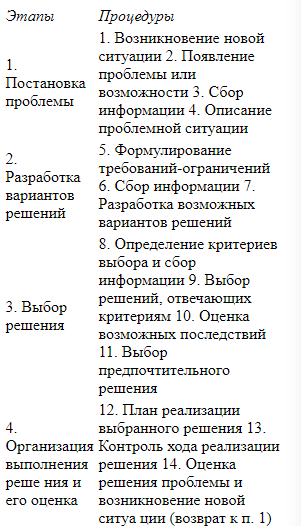
\includegraphics[width=\maxwidth{\textwidth}]{management-figures/phases_and_procedures_of_mananegent_decision}
	\caption{Этапы и процедуры процесса принятия решений}
\end{figure}

\subsection{Необходимость моделирования. Обзор моделей науки управления}
\textbf{Модель} – представление объекта системой или идеей в некоторой форме отличный от самой целостности. 
Существуют три базовых типа:
\begin{enumerate}
	\item Физическая модель – предтавляет то, что исследуется с помощью увеличенного описания объекта или системы.
	\item Аналагговая представляет объект аналогом, который ведет себя как реальный объект но не выглядит как таковой. 
	\item Математическая модель(символическая) – использует символы для описания свойств или характеристик объекта или события. 
\end{enumerate}

Этапы построения моделей:
\begin{enumerate}
	\item Постановка задачи
	\item Построение моделей
	\item Проверка моделей на достоверность
	\item Применение моделей и обновление ее.
\end{enumerate}

Причины обуславливающие необходимость моделирования:
\begin{enumerate}
	\item Естественная сложность многих организационных ситуаций.
	\item Невозможность проведения эксперимента в реальной жизни, даже когда они необходимы.
	\item Ориентация руководства на будущее.
\end{enumerate}

Наиболеей распростроненные виды моделей
\begin{enumerate}
	\item Модели теории игр (игры в конкуренцию, прогнозирование конкурента(
	\item Молели теории очередей или модели оптимального обслуживания (Как рассосать очередь в Макдаке в час пик( 
	\item Модель управления запасами (поддерживать температуру склады, борьба с грызунами, управление складированием)
	\item Модели линейного программирования
	\item Иммитационное моделирования – иммитация реальной системы 
	\item Модель экономического анализа (описание экономических показателей)
\end{enumerate}

\subsection{Общенаучные методы}
В процессе управления испоьзуется множество разнообразных способов, подходов и приемов, поволяющих упорядочить, целенапрпавить и эффективно организовать управление функции, этапов, процедур и операций необходимых для принятия решений. 
В совокупности они выступают как методы управления. 
Основу системы методов состовляяет общенаучная методология предусматривающая системный, комплексный подход к решению проблемы. 
А также применение такие методов, как моделирования, эксперемента, конкретно-исторический подход, экономико-математические и социологические исследования и т.д.
\begin{itemize}
	\item Системный подход применяется как способ упорядочения управленческих проблем, благодаря которому осуществляется их структурирование, определяются цели, решения, выбираются варианты, устанавливаются взаимосвязи и зависимости элементов проблем, а также факторы и условия, оказывающие воздействие на их решение.
	\item Комплексный подход являетя специфической формой конкретизации системности, так как его основу состовляет рассмотрение проблемы в их связи и их взаимозависимости с использованием методов исследования многих наук изучающих эти же проблемы. 
	\item Экономико-математические методы используются для решения задач оптимизации плана, формирования цен, распределения ресурсов и т.д.
	\item Эксперементирование --- экспреремент можно трактовать как научно поставленный опыт праводимый на базе разработанной методики, подготовленной специалистами с целью проверки тех или иных гипотез, нововведений и изменений в системе проектной деятельности. 
	Выделяют три результата:
	\begin{enumerate} 
		\item Об отрицательной оценке проверяемого нововведения.
		\item Формулировка, научное и практическое обоснование новых теоретических и методочиских положений наук и проблем. 
		\item Развитие системы методов управления.
	\end{enumerate}
	\item Конерктно-исторический подход --- подход, в соответствии рассматривается в динамике, поэтому при анализе проблем связанных с управлением важны такие параметры как время образования организации, основные события развития и т.д.
	\item Методы соц. исследований --- используется в решении проблем связанных с работающими, их ролью возникновений отклонений от запланированных целей, в выборе направления действий и заинтересованностью в выполнении намеченного плана мероприятия. 
\end{itemize}

\subsection{Конкретные или специфические методы управления}
Классификация конкретных методов осуществляется по трем основным направлениям, позволяющим выделить методы:
\begin{enumerate} 
	\item управления функциональными подсистемами;
	\item выполнения функций управления;
	\item принятия управленческих решений.
\end{enumerate}

\subsubsection{Методы управления функциональными подсистемами организации}
Первое направление связано со структурой организации, в которой имеется функциональное разделение управленческого труда по таким видам работ, как маркетинг, инновации, производство, финансы, персонал и т.п. 
Методы управления, применяемые в этих функциональных подсистемах, отражают их специфику в постановке целей и определении состава работ, необходимых для их выполнения. 
Они детально рассмотрены в главах, посвященных функциональному аспекту управления организациями.

Поэтому ограничимся лишь некоторыми примерами, характеризующими состав методов управления, используемых специалистами функциональных подсистем.

В подсистеме «Маркетинг» это методы:
\begin{itemize}
	\item диагностики положения организации на рынке товаров;
	\item анализа возможностей организации на потенциальных рын­ках;
	\item выявления потребностей в новых видах продукции и новых рынках сбыта;
	\item разработки маркетинговой концепции и т.д.
\end{itemize}

В подсистеме «Персонал» большое значение придается мето­дам:
\begin{itemize}
	\item анализа и формирования системы управления персоналом;
	\item планирования рабочей силы;
	\item организации труда персонала, его оплаты;
	\item управления деловой карьерой и др.
\end{itemize}

Управление подсистемой «Производство» требует применения большого количества самых разнообразных методов. В их числе методы:
\begin{itemize}
	\item анализа надежности;
	\item контроля качества;
	\item факторного анализа;
	\item функционального анализа;
	\item контроля использования труда, материалов, оборудования;
	\item изучения операций;
	\item программирования, планирования и контроля производства;
	\item учета расходов и др.
\end{itemize}

\subsubsection{Методы выполнения функций управления}
Методы управления, применяемые в различных функциональных подсистемах организации, связаны с выполнением функций, которые составляют содержание процесса управления. 
Поэтому, несмотря на специфику каждой подсистемы организации, в ней обязательно осуществляются такие действия, как планирование, организовывание, руководство и контроль. 
Этот подход заложен в основу второго направления классификации методов управления. 
Он позволяет сгруппировать и создать фонды методов, используемых организацией для выполнения любой из функций менедж­мента, вне зависимости от того, в какой подсистеме она реализу­ется.
Выполнение функции организовывания базируется на методах, позволяющих сформировать структуру организации, соответствующую стратегии ее развития и обеспечивающую эффективную совместную работу людей для достижения поставленных целей. 
Это прежде всего методы организационного проектирования, оценки сложности структуры, определения уровня формализации, делегирования полномочий, распределения обязанностей и ответ­ственности, реструктуризации, организации производства, труда и управления.

\subsubsection{Методы принятия управленческих решений}
Методы принятия управленческих решений --- третье направление классификации, которое базируется на представлении процесса управления как совокупности этапов и процедур, необходимых для разрешения проблем. 
В соответствии с этим выделяют группы методов: постановки проблемы; решения проблем; выбора решения; организации выполнения принятого решения.
Методы, используемые на этапе постановки проблемы или воз­можности, обеспечивают их достоверное и наиболее полное описание, выявление и анализ воздействия внутренних и внешних факторов, дают возможность оценить ситуацию и сформулировать на этом основании проблемную ситуацию. 
В их составе существенная роль принадлежит методам сбора, хранения, обработки и анализа информации, методам фиксации важнейших событий, факторного анализа, сравнения, аналогии, декомпозиции, моделирования, и т.п. 
Набор применяемых приемов зависит от характера и содержания проблемы, уровня ее появления и решения, сроков и средств, которые выделяются на этом этапе.

\subsection{Сущность и смысл контроля}
Слово <<контроль>> как и слово <<власть>> рождает прежде всего отрицательные эмоции. 
Для многих людей контроль означает прежде всего ограничение (как цепь для собаки), принуждение, отсутстзие самостоятельности и т.п. --- в общем, все то, что прямо противоположно нашим представлениям о свободе личности. 
Вследствие такого устойчивого восприятия, контроль относится к числу тех функций управления, сущность которых понимается чаще всего неправильно. 
Если спросить, что же означает контроль для менеджера, то чаще всего люди ответят вам, --- это то, что позволяет удерживать работников в определенных рамках. 
В принципе --- это верно. 
Один из аспектов контроля действительно состоит в обеспечении подчинения чему-то. 
Однако сводить контроль просто к неким ограничениям, исключающим возможность действий, наносящих вред организации и заставляющих каждого вести себя строго дисциплинированно, --- означало бы упустить из виду основную задачу управления.

Контроль --- это процесс обеспечения достижения организацией своих целей.
Процесс контроля состоит из установки стандартов, измерения фактически достигнутых результатов и проведения корректировок в том случае, если достигнутые результаты существенно отличаются от установленных стандартов.

Почему необходим контроль?

Руководители начинают осуществлять функцию контроля с того самого момента, когда они сформулировали цели и задачи и создали организацию. 
Контроль очень важен, если вы хотите, чтобы организация функционировала успешно. 
Без контроля начинается хаос и объединить деятельность каких-либо групп становится невозможно. 
Важно и то, что уже сами по себе цели, планы и структура организации определяют ее направление деятельности, распределяя ее усилия тем или иным образом и направляя выполнение работ. Контроль, таким образом, является неотъемлемым элементом самой сущности всякой организации. 
Это и дало основание Питеру Друкеру заявить: <<Контроль и определение направления --- это синонимы>>.

\subsection{Процесс контроля}
В процессе контроля выделяют 3 этапа:
\begin{enumerate}
	\item выработка стандартов и критериев;
	\item сопоставление с ними реальных результатов;
	\item принятие необходимых корректирующих действий.
\end{enumerate}

\subsubsection{1 этап - Установление стандартов}
Стандарты --- это конкретные цели, поддающиеся измерению. 
Все стандарты, которые используются для контроля, выбираются из многочисленных целей и стратегий организации.
Цели, которые могут быть использованы в качестве стандартов для контроля имеют 2 особенности:
\begin{enumerate}
	\item имеют временные рамки, в которых должна быть выполнена работа;
	\item имеют конкретный критерий, по отношению к которому можно оценить степень выполнения работы.
\end{enumerate}

Стандарты устанавливаются в форме показателей результативности, которые точно определяют то, что должно быть получено для того, чтобы достичь поставленных целей. Например, легко установить показатели результативности для таких величин как объем продаж, прибыль и другие, т. к. они поддаются количественному измерению. 
Но очень сложно и часто вообще невозможно выразить в числовых показателях, например, повышение морального уровня сотрудников организации, рассматриваемое в качестве цели.

\subsubsection{Сопоставление достигнутых результатов с установленными стандартами}
На данном этапе менеджер должен определить, насколько достигнутые результаты соответствуют его ожиданиям. 
Кроме того, здесь принимается еще одно важное решение - насколько допустимы и безопасны обнаруженные отклонения от стандартов. 
Деятельность, осуществляемая на этой (второй) стадии контроля, является наиболее заметной частью всей системы контроля. 
Эта деятельность состоит в определении масштаба отклонений, измерении результатов, передаче информации и ее оценке.

Руководство высшего звена устанавливает масштаб допустимых отклонений, в пределах которого отклонение полученных результатов от намеченных не должно вызывать беспокойство.

Одним из способов возможного увеличения экономической эффективности контроля является использование метода управления по принципу исключения. 
Принцип исключения состоит в том, что система контроля должна срабатывать только при наличии замеченных отклонений от стандартов.

Измерение результатов --- самый сложный и дорогостоящий элемент контроля. 
Чтобы быть эффективной, система измерения должна соответствовать тому виду деятельности, который контролируется.

Чтобы система контроля действовала эффективно, надо обязательно довести до сведения соответствующих работников организации как установленные стандарты, так и достигнутые результаты. 
Кроме того, должна быть обеспечена эффективная связь между теми, кто устанавливает стандарты и теми, кто должен их выполнять.

\subsubsection{Выбор подходящей линии поведения}
На данном этапе менеджер должен выбрать одну из трех линий поведения:
\begin{enumerate}
	\item ничего не предпринимать (если сопоставление фактических результатов со стандартами говорит о том, что установленные цели достигаются, лучше всего ничего не предпринимать);
	\item Устранить отклонения (проводимая корректировка должна концентрироваться на устранении настоящей причины отклонения. 
	Смысл корректировки состоит в том, чтобы понять причины отклонения и добиться возращения организации к правильному образу действия);
	\item пересмотр стандартов (не все замеченные отклонения от стандартов следует устранять. 
	Иногда сами стандарты могут оказаться нереальными, потому что они основываются на планах, а планы --- это прогнозы будущего. 
	При пересмотре планов должны пересматриваться и стандарты).
\end{enumerate}

\subsection{Характеристики эффективного контроля}
Все эффективные системы контроля имеют общие требования. 
Их значимость варьируется в зависимости от конкретной ситуации, однако мы можем с уверенностью сказать, что если контроль соответствует требованиям, то его эффективность значительно повышается. 
Рассмотрим каждое требование.
\begin{enumerate}
	\item \textbf{Действенность.} 
	Выявленные в результате контроля нарушения, изъяны, ошибки, промахи в деятельности предприятия (организации) должны оперативно устраняться.
	\item \textbf{Гибкость.} 
	Эффективные контрольные механизмы должны предотвращать последствия неблагоприятных изменений и учитывать преимущества новых возможностей. 
	Очень немногие современные организации работают в условиях стабильной внешней среды и не нуждаются в гибкой системе контроля. 
	Сегодня даже самые механистические структуры требуют механизмов контроля, которые можно скорректировать в соответствии с изменением ситуации и обстановки.
	\item \textbf{Систематичность.} Контроль должен проводиться не от случая к случаю, а постоянно. 
	Кроме этого все виды и процедуры контроля, осуществляемые в организации, должны быть связаны в единую взаимозависимую целостность.
	\item \textbf{Комплексность.} 
	Контроль должен охватывать не один или несколько показателей плана, а все показатели, все направления деятельности предприятия (организации). 
	Реализация контрольной функции в организации всегда должна быть единым комплексом, а не набором случайно связанных или вообще не связанных процедур.
	\item \textbf{Экономичность.} 
	Эффективная система контроля должна оправдывать издержки, связанные с ее созданием и применением. 
	Чтобы минимизировать эти затраты, менеджерам следует использовать как можно меньше контрольных механизмов, т.е. внедрять только те методики и способы, которые действительно необходимы для достижения намеченных результатов. 
	Выгоды, приносимые контролем, должны быть выше затрат на его проведение.
	\item \textbf{Гласность.} 
	Результаты контроля должны быть известны исполнителям.
	\item \textbf{Своевременность.} 
	Механизмы контроля должны своевременно привлекать внимание менеджера к отклонениям, чтобы он мог предупредить их серьезное влияние на работу подразделения. Даже самые ценные сведения обесцениваются, если поступают с опозданием. 
	Следовательно, эффективная система контроля должна обеспечивать своевременную информацию.
	\item \textbf{Понятность.} Механизмы контроля, непонятные для тех, кто ими пользуется, бессмысленны. 
	По этой причине иногда возникает необходимость упростить систему контроля. 
	Применение системы контроля, которую трудно понять, нередко приводит к дополнительным ошибкам, недовольству сотрудников и к тому, что люди их просто игнорируют.
	\item Самым главным фактором повышения эффективности контроля, а значит, и изменения характера управления является \textbf{развитие партнерства} – управления, осуществляемого на основе участия всех членов организации или группы в управлении.
	 Для такого совместного управления характерно внедрение и развитие \textbf{самоконтроля}.
\end{enumerate}

%
% section 2
%
\section{Модуль II}
\subsection{Концепция управления персоналом}
Основу концепции управления персоналом органиpации в настоящее время составляет возрастающая роль личности работника, знания его мотивационных установок, умение их формировать и направлять в соответствии с задачами стоящими перед организациями. 
Укрупненно можно выделить три фактора оказывающих воздействие на людей в организации:
\begin{enumerate}
	\item Иерархичсеская структура организации
	\item Культура
	\item Рынок
\end{enumerate}
Эти факторы воздействия --- факторы достаточно сложные и на практике редко реализуются по отдельности. 
От того, какому из них отдается приоритет зависит облик ситуации в организации.
Структура службы во многом зависит от характера и размера организации, особенностей выпускаемой продукции или оказания услуг.
В мелких и средних организациях многие функции по управлению персонала выполняются преимущественно линейными руководителями, а в крупных формируется самостоятельные структурные подразделения по реализации функций.

\subsection{Принципы управления персоналом}
\begin{itemize}
	\item принципы характеризующие требования к формирования ситемы управления персоналом;
	\item приниципы определяющие направление развития системы управления персоналом.
\end{itemize}
Все принципы построения системы управления персоналом реализуются во взаимодействии. Их сочетание зависит от конкретных условий функционирования.

\subsection{Методы построения системы управления персоналом (СУП)}
Методы анализа и построения СУП: 
\begin{enumerate}
	\item \textbf{Системный анализ} \\ 
	Рассматривается в качестве методического средства системного подхода к эффективному решению проблем для совершенствования системы управления персоналом. 
	Роль системного подхода состоит в ориентировании сотрудников как на реализацию в целом рассматриваемого проекта, так и его составляющих задач, к которым относят: цели, функции, организационную структуру, кадры, технические средства управления, информацию, методы управления персоналом, управленческие решения.
	Благодаря этому подходу выявляются многообразные типы связей между внутренними данными и внешней средой, сведение их в целостно-единую картину.
	\item \textbf{Метод декомпозиции} \\ 
	Содействует разделению сложных задач на более простые.
	При большей простоте элементов достигается более полное проникновение в самую суть процесса, и выявление сущности этой задачи. 
	Так, система управления персоналом может быть разделена на подсистемы. 
	Подсистемы подразделяются на функции. 
	Функции дробятся на процедуры. 
	Процедуры делятся на операции.
	\item \textbf{Метод последовательной подстановки} \\ 
	С его помощью реально исследовать влияние каждого из отдельных факторов развития организации на формирование системы управления персонала при воздействия внешних факторов.
	\item \textbf{Метод структуризации целей} \\ 
	Данному методу присуще: осуществление обоснования целей организации \textit{(количественного и качественного)}; проверку целей системы управления персоналом с точки зрения их соответствия целям организации. 
	Построение рациональной системы управления персоналом организации невозможно без анализа целей, развёртывания их иерархически, установления ответственности каждого из сотрудников за конечные результаты работы, определения их места в системах производства и менеджмента, устранения дублирования в работе персонала.
	\item \textbf{Экспертно-аналитический метод} \\ 
	Предусматривает привлечение к решению задач по совершенствованию управления персоналом на предприятии высококвалифицированных специалистов в качестве экспертов. 
	Они дают оценки существующего положения, устанавливают недостатки по работе сотрудников и их причины.
	Имеющиеся у экспертов единые критерии нередко отсутствуют, из-за чего метод страдает невысокой объективностью и точностью. 
	Для получения более объективных оценок практикуется использование многошаговой экспертизы.
	\item \textbf{Нормативный метод} \\ 
	Основан на применении системы нормативов, которые дают ориентиры содержанию и структуре функций, касающихся управления персоналом, численности персонала, типу организационной структуры аппарата управления \textit{(и организации в целом, и системы управления персоналом)}, кооперации и разделению труда специалистов и руководителей в области управления организацией.
	\item \textbf{Параметрический метод} \\ 
	Он предполагает определение степени соответствия параметров системы управления персонала параметрам производственной системы предприятия посредством установления функциональных зависимостей между ними.
	\item \textbf{Метод функционально-стоимостного анализа} \\ 
	С его помощью реально осуществить выбор такого варианта построения системы управления персоналом, который будет наименее затратным и эффективным с позиции достижения конечных результатов в работе предприятия. 
	При его реализации выявляются как лишние, так и дублирующие управленческие функции, функции, не выполняющиеся \textit{(по конкретным причинам)}, определяется степень централизации/децентрализации функций по управлению персоналом.
	\item \textbf{Метод главных компонентов} \\
	Дает возможность отражения в одном единственном компоненте \textit{(показателе)} свойства многих. 
	Это способствует упрощению сравнения ряда систем управления персоналом.
	\item \textbf{Балансовый метод} \\ 
	Способствует осуществлению балансовых сопоставлений, увязки, к примеру, при сопоставлении итогов обработки фотографий рабочего дня и технологических карт выполнения операций управления с реальным временем их выполнения.
	\item \textbf{Корреляционный и регрессионный анализ} \\ 
	Устанавливает зависимость и тесноту связи между численностью работников и факторами, которые воздействуют на нее.
	\item \textbf{Опытный метод} \\ 
	Основан на изучении опыта предшествующих периодов в работе предприятия и опыта иных подобных систем.
	\item \textbf{Метод аналогий} \\
	Базируется на исследовании оправдавших себя организационных форм управления персоналом. 
	Суть метода состоит в опоре на типовые решения \textit{(к примеру, решения по организационной структуре предприятия)}, которые разрабатываются в целях последующего развития бизнеса.
	\item \textbf{Метод творческих совещаний} \\ 
	Предусматривает коллективное \textit{(групповое)} рассмотрение эффективности направлений развития системы управления персоналом рядом руководителей. 
	При применении этого метода используется потенциал потока идей и выявляются варианты способов совершенствования системы управления персоналом.
	\item \textbf{Метод коллективного блокнота} \\ 
	Даёт возможность \textit{(при поиске путей совершенствования системы управления персоналом)} сочетания независимого выдвижения идей специалистами-экспертами с их коллективной оценкой в условиях совещания.
	\item \textbf{Метод контрольных вопросов} \\ 
	Предполагает активизацию творческого поиска оптимального решения проблемы, связанной с совершенствованием системы управления персоналом, посредством наводящих вопросов, которые подготавливаются заранее соответствующими службами.
	\item \textbf{Метод 6-5-3} \\
	Предназначен для систематизации процесса нахождения идей по развитию системы управления персоналом. 
	Суть этого метода заключается в том, что каждый их шести членов экспертной группы пишет на отдельном листе бумаги по три идеи и передает их остальным членам группы, которые, в свою очередь, на основе уже предложенных вариантов пишут еще по три идеи, и т.д. 
	По окончании этой процедуры на каждом из шести листов будет записано по 18 вариантов решений, а всего будет 108 вариантов.
	\item \textbf{Морфологический анализ} \\ 
	Средство изучения всевозможных комбинаций вариантов организационных решений предлагаемых для осуществления отжельных функций управления персоналом. 
	Если записать столбиком все функции, затем против каждой функции указат все возожные варианты, то получим морфологическую таблицу. 
	Идея: разбить сложную задачу на мелкие, при этом предполагается.
\end{enumerate}

\subsection{Методы управления персоналом}
Методами управления персоналом называют способы воздействия на коллективы и отдельных работников с целью осуществления координации их деятельности в процессе производства.
Экономические методы управления --- связаны с использованием средств и иструментов экономической заинтересованности управляемого объекта в решении тех или иных задач без мер административного воздействия. 
При экономических методах управления произодство гибче и быстрее реагирует на изменение общественных потребностей. 
Инструментами экономческких методов управления являются такие рычаги воздействия как: 
\begin{itemize}
	\item цены;
	\item кредит;
	\item стоимость;
	\item зарабатная плата.
\end{itemize}
Административные методы --- предполагают пряиое воздействие на управляемый объект. 
С их помощь осуществляется правовые функции входящие в круг обязанностей управленческих органов и предусмотренные соответствующими официальными положениях предприятий, а также должностными инструкциями.
Социально-психологические методы упраления --- основаны на социальном организме, социальных потребностях и взаимоотношениях в коллективе. 

\subsection{Источники организации найма персонала}
Набор заключается в создании необходимого резерва кандидатов на все должности,на которые организации выбирают наиболее подходящих. 
Имеются два основных источника набора:
\begin{itemize}
	\item \textbf{Внутренний} \\[0.5em]
	\begin{tabularx}{\linewidth}{|X|X|}
		\hline
		Преимущества & Недостатки \\ \hline
		\begin{itemize}[leftmargin=*, topsep=0pt]
			\item работники видят пример;
			\item лучшие возможности оценки работы;
			\item сокращение затрат на наём, так как компания знает достоинтсва и недостатки.
		\end{itemize}
		& 
		\begin{itemize}[leftmargin=*, topsep=0pt]
			\item угроза накопления плохих взимоотношениях в работе;
			\item семейственность;
			\item плохое отношение к человеку со стороны его бывших коллег.
		\end{itemize} \\ \hline
	\end{tabularx} \\[0.5em]
	\item \textbf{Внешний} \\[0.5em]
	\begin{tabularx}{\linewidth}{|X|X|}
		\hline
		Преимущества & Недостатки \\ \hline
		\begin{itemize}[leftmargin=*]
			\item выбор из большого числа кандидатов
			\item меньшая угроза возникновения интриг
		\end{itemize}
		& 
		\begin{itemize}[leftmargin=*]
			\item долгий период привыкания;
			\item ухудшение морального климата среди давноработающих;
			\item рабочие <<хватки>> новых сотрудников заранее не известны.
		\end{itemize} \\ \hline
	\end{tabularx} \\[0.5em]
\end{itemize}
К средствам внешнего набора относятся: публикация объявлений в газетах и проф. журналах. 
Обращение к агентам по трудойстройству, направление заключивших контракт людей на специальные курсы. 
Дополнительные источники: 
\begin{itemize}
	\item бывшие сотрудники;
	\item случайные претенденты;
	\item институты;
	\item колледжи;
	\item клиенты и поставщики.
\end{itemize} 
Рекламные объявления должны содержать информацию о ключевых эдементах работы, требуемой квалификации, местонахождении, уровне и зарплате.

\subsection{Требования к кандидатам на замещение вакантной должности}
\begin{enumerate}
	\item Проверка претендентов с использованием ряда формальных методов:
	\begin{enumerate}
		\item Опытными специалистами и руководителями 
		\item Замещение молодыми специалистами, выпускниками вузов.
		\item Продвижение на вышестоящую должность изнутри.
	\end{enumerate}
	\item При подборе персонала:
	\begin{itemize}
		\item образование;
		\item особенности инетелекта;
		\item основные особенности интереса.
	\end{itemize}
	\item Тестирование:
	\begin{itemize}
		\item тех. тестирование на знание основ и приемов;
		\item психологическое тестирование.
	\end{itemize}
	\item Коммуникативное тестировавние \textit{(социальные качества)}.
	\item Писменные задания.
	\item Устные экзамены.
\end{enumerate}
Также получили развитие такие виды совместимости:
\begin{itemize}
	\item Графологические
	\item Полиграф
	\item Астрология
	\item Херомантия
	\item Физиогномика
	\item Пластика
\end{itemize}

\subsection{Организация процесса отбора претендентов на вакантную должность}
% http://www.strategplann.ru/uskorennoe-formirovanie-kollektiva/organization-of-selection-of-candidates-for-the-vacant-post.html
Конечное решение при отборе обычно формируется на несколь­ких этапах, которые следует пройти претендентам. 
На каждом эта­пе отсеивается часть претендентов или же они отказываются от процедуры, принимая другие предложения.
\begin{enumerate}
	\item \textbf{Предварительная отборочная беседа}.
	\item \textbf{Анкетирование} \\
	Наряду с решением задач отсева менее подходящих кандидатов определяется круг факторов, нуждающихся в особо пристальном изучении на основе последующих методов, а также источники, из которых можно получить необходимую информацию. 
	Любое ее искажение в анкете является основанием для увольнения работника в любой момент, когда это выяснится.
	Анализ анкетных данных в сочетании с другими методами отбора выявляет следующее:
	\begin{itemize}
		\item соответствие уровня образования заявителя минимальным квалификационным требованиям;
		\item соответствие практического опыта характеру должности;
		\item наличие ограничений иного рода на выполнение должностных обязанностей;
		\item готовность к принятию дополнительных нагрузок (сверхурочные работы, командировки);
		\item круг лиц, которые могут рекомендовать работника, помочь наведению справок и получению дополнительной информации.
	\end{itemize}
	\item \textbf{Собеседование}.
	\item \textbf{Тестирование}.
	\item \textbf{Медицинский осмотр} \\ 
	Некоторые организации требуют, чтобы наиболее подходящие им заявители заполняли медицинские вопросники или проходили медицинский осмотр. 
	Причины для такого требования следующие:
	\begin{itemize}
		\item в случае подачи работниками жалоб по поводу компенсации необходимо знание физического состояния заявителя в момент найма;
		\item необходимо предотвратить наем переносчиков заразных болезней.
	\end{itemize}
\end{enumerate}

\subsection{Сущность и виды профориентации и адаптации персонала}
% http://www.strategplann.ru/uskorennoe-formirovanie-kollektiva/nature-and-types-of-guidance-and-adaptation-of-staff.html
Профессиональная ориентация представляет собой систему мер по профинформации, профконсультации, профподбору и профадаптации, которая помогает человеку выбирать профессию, наиболее соответствующую потребностям общества и его личным способностям и особенностям.

Цель профориентации --- оказание помощи молодым людям и людям, ищущим работу, в выборе профессии, специальности, нахождении места работы или учебы с учетом склонностей и интересов.

Задачи профориентации --- информирование заинтересованных лиц о видах профессиональной деятельности.

Трудовая адаптация персонала --- взаимное приспособление работника и организации, основывающееся на постепенном включении работника в процесс производства в новых для него профессиональных, психофизиологических, социально-психологических, организационно-административных, экономических, санитарно-гигиенических и бытовых условиях труда и отдыха.

Выделяют два направления трудовой адаптации: первичную и вторичную.

Принципиальные цели адаптации можно свести к следующему:
\begin{itemize}
	\item уменьшение стартовых издержек, так как пока новый работник плохо знает свое рабочее место, он работает менее эффективно и требует дополнительных затрат;
	\item снижение степени озабоченности и неопределенности у новых работников;
	\item сокращение текучести рабочей силы, так как если новички чувствуют себя неуютно на новой работе и ненужными, то они могут отреагировать на это увольнением;
	\item экономия времени руководителя и сотрудников, так как проводимая по программе работа помогает экономить время каждого из них;
	\item развитие позитивного отношения к работе, удовлетворенности работой.
\end{itemize}

Выделяют два направления трудовой адаптации: первичную и вторичную.

В условиях функционирования рынка труда возрастает роль вторичной адаптации. 
При этом необходимо внимательно изучать опыт зарубежных фирм, которые уделяют повышенное внимание первичной адаптации молодых работников. 
Данная категория персонала нуждается в особой заботе со стороны администрации организаций. 
Чаще всего профессиональная адаптация рассматривается как процесс приобщения человека к труду в рамках определенной профессии, включения его в производственную деятельность, усвоения им условий и достижения нормативов эффективности труда. 
Однако адаптацию нельзя рассматривать только как овладение специальностью. 
Она предусматривает также приспособление новичка к социальным нормам поведения, действующим в коллективе, установление таких отношений сотрудничества работника и коллектива, которые в наибольшей мере обеспечивают эффективный труд, удовлетворение материально-бытовых и духовных потребностей обеих сторон.
Принципиальные цели адаптации можно свести к следующему:
\begin{itemize}
	\item уменьшение стартовых издержек, так как пока новый работник плохо знает свое рабочее место, он работает менее эффективно и требует дополнительных затрат;
	\item снижение степени озабоченности и неопределенности у новых работников;
	\item сокращение текучести рабочей силы, так как если новички чувствуют себя неуютно на новой работе и ненужными, то они могут отреагировать на это увольнением;
	\item экономия времени руководителя и сотрудников, так как проводимая по программе работа помогает экономить время каждого из них;
	\item развитие позитивного отношения к работе, удовлетворенности работой.
\end{itemize}
Отметим, что в отечественных организациях наблюдается не отработанность механизма управления процессом адаптации. Этот механизм предусматривает решение трех важнейших проблем:
\begin{itemize}
	\item структурного закрепления функций управления адаптацией в системе управления организацией;
	\item организации технологии процесса адаптации;
	\item организации информационного обеспечения процесса адаптации. 
	Структурное закрепление функций управления адаптацией может проходить по следующим направлениям.
	\begin{enumerate}
		\item Выделение соответствующего подразделения (бюро, отдела) в структуре системы управления персоналом. 
		Чаще всего функции по управлению адаптацией входят в состав подразделения по обучению персонала.
		\item Распределение специалистов, занимающихся управлением адаптацией, по производственным подразделениям организации, координации их деятельности со стороны службы управления персоналом.
		\item Развитие наставничества, которое в последние годы в отечественных организациях незаслуженно забыто.
	\end{enumerate}
\end{itemize}
Успешность адаптации зависит от целого ряда условий, в том числе:
\begin{itemize}
	\item качественный уровень работы по профессиональной ориентации потенциальных сотрудников;
	\item объективность деловой оценки персонала (как при отборе, так и в процессе трудовой адаптации работников);
	\item отработанность организационного механизма управления процессом адаптации;
	\item престиж и привлекательность профессии, работы по определенной специальности именно в данной организации;
	\item особенности организации труда, реализующие мотиваци-онные установки сотрудника;
	\item Наличие отработанной системы внедрения новшеств;
	\item гибкость системы обучения персонала, действующей внутри организации;
	\item особенности социально-психологического климата, сложившегося в коллективе;
	\item личностные свойства адаптируемого сотрудника, связанные с его психологическими чертами, возрастом, семейным положением и т.п.
\end{itemize}

\subsection{Опыт профориентации и адаптации персонала}
\subsubsection{Опыт Японии}
Система подготовки кадров здесь отличается большой спецификой. 
Учащиеся японской школы до перехода на вторую ступень среднего образования (10-12 классы) практически не могут получить какой-либо профессиональной подготовки, т.е. большая часть японской молодежи, имея среднее образование, выходит на рынок труда если не вовсе профессионально не подготовленной, то во всяком случае без какого-либо свидетельства о присвоении квалификации. 
Это, однако, мало смущает руководство японских компаний.

Профессиональная подготовка в фирмах --- неотъемлемая часть японской системы управления кадрами. 
Руководство компаний стремится привлечь молодых людей непосредственно со школьной скамьи, потому что отсутствие каких-либо навыков в работе свидетельствует о неиспорченности, отсутствии стороннего влияния, готовности воспринять правила поведения, принятие в данной корпорации. 
Поступившая молодежь проходит обязательный курс начальной подготовки --- адаптации. 
Это происходит в течение относительно короткого периода --- двух месяцев. 
Основной смысл начального обучения --- знакомство новичков с компанией, принципами взаимоотношений сотрудников, традициями, обычаями, ритуалами, т. е. в моральной подготовке к работе.

\subsubsection{Опыт США}
Углубленные программы адаптации работников применяются на средних и крупных фирмах США. 
В процессе их проведения участвуют как менеджеры по управлению персоналом, так и линейные менеджеры. 
На малых предприятиях программа адаптации проводится менеджером-практиком, иногда с включением работника профсоюза, используются самые различные программы --- от программ, предусматривающих, в основном, устную информацию, до формализованных процедур, связывающих устные представления с письменными и графическими установками. 
В формальных программах адаптации часто используют аппаратуру, слайды, фотографии. 
Программы подразделяются на общие и специализированные. Как правило, вопросы общей программы касаются информации о предприятии в целом. 
Вот некоторые вопросы, затрагиваемые этой программой: 
\begin{itemize}
	\item общее представление о компании, приветственная речь, цели, приоритеты, традиции, нормы, продукция, виды деятельности, данные о руководстве, внутренние отношения; 
	\item ключевая политика; 
	\item оплата труда; 
	\item дополнительные льготы; 
	\item охрана труда и техника безопасности; 
	\item работник и его отношения с профсою­зом; 
	\item служба быта; 
	\item экономические факторы: прибыль, стоимость рабочей силы, стоимость оборудования, ущерб от прогулов, опозданий, несчастных случаев.
\end{itemize}

\subsection{Организация управления профориентацией и адаптацией персонала}
Управление профессиональной ориентацией и адаптацией строится через формирование и развитие системы органов управления различного уровня.

Вопросами адаптации занимаются отдельные работники из разных подразделений: менеджер по персоналу, линейные руководители или коллеги по работе. 
Их главная цель --- сделать процесс адаптации приспособления молодых работников к предприятию как можно более коротким и безболезненным. 
Необходимо отметить, что процессы как первичной, так и вторичной адаптации значительно не отличаются.

Процесс адаптации непосредственно начинается в отделе кадров при приеме и оформлении на работу. 
Инспектор отдела кадров проводит небольшую беседу, в которой в общих чертах знакомит с предприятием, отделом или цехом, где предстоит работать новичку. 
Затем он провожает нового работника на его рабочее место и представляет непосредственному руководителю. 
А тот, в свою очередь, знакомит с коллективом, коллегами по работе, с рабочим местом. 
По своему усмотрению руководитель может прикрепить к новичку наставника из числа более опытных и старших работников. 
Как правило, еще в течение месяца руководитель проводит периодические беседы с новым работником, интересуясь трудностями, которые у него возникают, его успехами, и систематически оценивает его работу. 
Контроль за ходом процесса адаптации со стороны отдела кадров не проводится.

\begin{figure}[h]
	\centering
	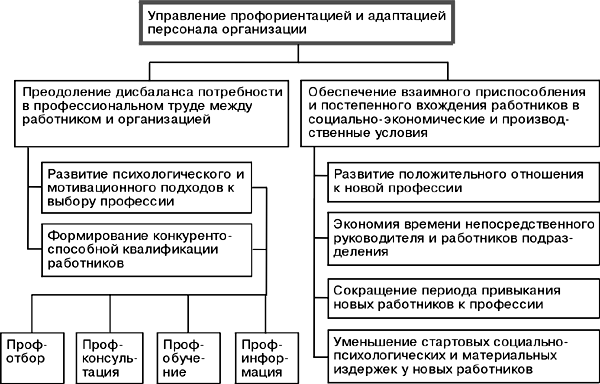
\includegraphics[width=\maxwidth{\textwidth}]{management-figures/adapt_goal}
	\caption{Цели и задачи системы управления профориентацией и адаптацией персонала в организации}
\end{figure}

Подразделение по управлению профориентацией и адаптацией должно выполнять следующие функции:
\begin{itemize}
	\item изучение и прогнозирование конъюнктуры рынка труда, проведение мероприятий по адаптации к нему, осуществление соответствующей переструктуризации кадрового потенциала;
	\item наем и отбор персонала с использованием профессиограмм и описаний работ, тестирования и интервьюирования работников с целью их лучшей профориентации;
	\item расстановка кадров по подразделениям, участкам, рабочим местам, закрепление ротаций и внутрипроизводственные перемещения кадров, формирование стабильного трудового коллектива;
	\item отбор лидеров из числа молодых работников, обладающих талантом организатора;
	\item организация взаимодействия с региональной системой управления профориентацией и адаптацией на взаимовыгодных условиях.
\end{itemize}

В обязанности менеджера по персоналу входят:
\begin{itemize}
	\item ознакомление с организацией, характеристика условий найма, оплаты труда;
	\item представление руководителю, непосредственному начальнику, инструктору по обучению;
	\item организация экскурсии по рабочим местам;
	\item разъяснение условий работы, ознакомление с функциями (совместно с руководителем);
	\item организация обучения (совместно с отделом обучения);
	\item введение в коллектив, представление сотрудников (совместно с руководителем).
\end{itemize}

\subsection{Изучение состояния работы по профориентации и адаптации персонала}
Сбор информации о состоянии профориентации и адаптации в организации следует проводить по результатам обработки специально разработанного вопросника для изучаемой категории работников.

Пример анкеты:
\begin{enumerate}
	\item Ваше место работы или учебы до поступления в организацию.
	\item Кто повлиял на ваш выбор профессии?
	\item В какие периоды вам наиболее необходима помощь руководителя?
	\item Как часто вам нужна в работе помощь коллег?
	\item В какой период вашей деятельности вы почувствовали в себе профессиональные навыки?
	\item В какой период вы почувствовали, что вошли в коллектив?
	\item Устраивает ли вас занимаемое место в коллективе?
	\item Представьте себе, что по каким-либо причинам вы уволились из организации. 
	Вернулись ли бы вы через некоторое время на свое прежнее место работы?
	\item Бывают ли у вас конфликты.
	\item Кто оказал вам наиболее ощутимую помощь в процессе адаптации: сотрудник отдела кадров, линейный руководитель, наставник, коллега по работе или кто-то еще? 
	\item Что помогло вам в процессе адаптации: лекции, семинары, специальная литература, фильмы, слайды?
\end{enumerate}

\subsection{Группы и их значимость}
Существуют три основные типы групп:
\begin{itemize}
	\item Группы руководителей как сопадчиненных команд на разных уровнях управления
	\item Группы рабочих (целевая рабочая группа).
	\item Группы комитетов, советов и коммиссий (группы внутри организации, которым деллегированные полномочия для выполнения каких-то обобщенных задач)
\end{itemize}

\subsection{Управление неформальной организацией }
Неформальные группы --- это спонтанно образующиеся группы людей, которые вступают в регулярные взаимодействия параллельно с формальными группами и у них имеется поставленная цель, это дружественные группы основанные на контрактах и дружественных интересах. 
Особенно благоприятно для неформальных групп трудовая среда. 
Принадлженость к неформальной группе может положительно влиять на трудовую деятельность. 
Принадлежность к неформальным группам может дать людям психологические выводы, не менее важные для них, чем получения зарплаты. 
Для этого необходимо признать неформальные группы, выслушать требования членов и лидеров неформалных организаций, предполагать неблагоприятные воздействия на неформальную группу и разрешить принимать участие в разработке решений. 

\subsection{Повышение эффективности работы групп. Факторы, влияющие на эффективность деятельности групп и организации}
Решая проблемы управления группами руководство организации, как правило, решает проблемы повышения эффективности управления коллективом в целом. 
Основное внимание при этом должно уделяться определению ню основных показателей групп и факторов, на них влияющих:
\begin{itemize}
	\item \textbf{Размер группы} \\
	Идеальная группа 5-9 человек. 
	Увеличение размера группы ведет к ее неформального распределения и сложностей в управлении.
	\item \textbf{Состав группы} \\
	Степень сходства личностей и точек зрения при принятии решений. 
	Рекомендуют, чтобы группа состояла из неподобных личностей.
	\item \textbf{Групповое поведение} \\
	Наличие определенных правил и норм поведения, которых рекомендуют придерживаться, чтобы избежать возникновения конфликтных ситуаций.
	\item \textbf{Сплоченность} \\
	Мира тяготения членов группы друг к другу и к группе в целом. 
	Следует поддерживать.
	\item \textbf{Групповая единодушие} \\
	Тенденция к подавление отдельной личностью разных взглядов членов группы. 
	Следует избегать.
	\item \textbf{Конфликтность} \\
	Возможность возникновения внутригрупповых споров и конфликтов. 
	Рекомендуется использовать различные методы управления конфликтной ситуацией.
	\item \textbf{Статус членов группы} \\
	Старшинство в должности, название должности, размещение кабинета, образование, социальный талант, информированность и накопленный опыт. 
	Необходимо учитывать возможность как положительного так и отрицательного влияния статуса у отдельных лиц на членов группы и группы в цилому.
	\item \textbf{Роли членов группы} \\
	Характер поведения каждого члена группы.
	Существуют целевые, поддерживающие и отрицательные роли.
\end{itemize}

\subsection{Власть, влияние}
Повсеместно признается, что влияние и власть в равно степени зависит от личности, на которую оказывается влияние, а также от ситуации и способности руководителя.
\begin{description}
\item[Власть] Возможность влиять на поведение других.
\item[Влияние] Любое поведение одного индивида, которое вносит изменения в поведение, отношение, ощущение другого индивида.
\end{description}

Не существует реальной абсолютной власти.

Зачастую руководитель имеет власть над подчиненными потому что они зависят от него по работе. 
В отдельных ситуациях подчиненный имеет власть над руководителем, так как последних зависит от них в вопросах принятия решений, неформальных контактов, которые подчиненные могут оказывать на коллег и способность подчиненных выполнять задания. 

Формы власти:
\begin{enumerate}
	\item Власть, основанная на \textbf{принуждении} \textit{(исполнитель верит, что влияющий имеет возможность его наказывать)}.
	\item Власть, основанная на \textbf{вознаграждении}.
	\item \textbf{Экспертная} власть \textit{(исполнитель верит, что эксперт знает лучше)}.
	\item \textbf{Эталонная} власть.
	\item \textbf{Законная} власть \textit{(традиционная; исполнитель верит, что он имеет право приказывать)}.
\end{enumerate}

\subsection{Убеждение и участие}
% http://www.profession-in-perspective.org.ua/vliyanie.-ubezhdenie-i-uchastie,-kak-perspektivnye-formy-vliyaniya/
Базируется на умении руководителя эффективно передавать подчиненным свою точку зрения на способы решения любых проблем. 
Руководитель, который влияет путем убеждения, не указывает исполнителю, что следует сделать. 
Он доводит до сознания исполнителя что, сделав так, как этого хочет руководитель, исполнитель удовлетворит своего собственную потребность. 
В этом заключается сущность убеждения.

При этом руководитель допускает ситуации, при которых исполнитель владеет какой-то частью власти, которая уменьшает возможности руководителя действовать. Иначе говоря, руководитель признает своего независимость от исполнителя.

Эффективность влияния путем убеждения зависит от ряда факторов:
\begin{itemize}
	\item руководитель должен пользоваться доверием;
	\item аргументация руководителя должна учитывать интеллектуальный уровень работников;
	\item цель, которую ставит перед собой руководитель, не должна противоречить системе ценностей работников.
\end{itemize}

Современная практика менеджмента предусматривает такие методы влияния на работников путем убеждения:
\begin{itemize}
	\item пытайтесь как можно точнее определить потребности работника и апеллировать к этим потребностям;
	\item начинайте разговор из такой мысли, который обязательно его заинтересует;
	\item постарайтесь создать образ, который вызывает большое доверие и ощущение надежности;
	\item ведите разговор, исходя из интересов работника, а не своих собственных;
	\item если высказывается несколько точек зрения, пытайтесь высказываться последним; аргументы, которые выслушаны последними, имеют наибольший шанс повлиять на работников.
\end{itemize}

Наибольшее преимущество использования убеждения заключается в том, что произведенную работу не надо проверять, поскольку она удовлетворяет личные потребности человека, на которого направленное убеждение. 
При этом недостатками являются: медленное действие убеждения; неопределенность результатов; сложность применения такого подхода.

\subsection{Основы лидерства}
Лидерство --- это высшее проявление менеджмента.

Интеллектуальными людьми невозможно управлять. 
Творческие команды можно только направлять и вести.

Лидер должен получить признание команды. 
Для того этого необходимо:
\begin{enumerate}
	\item Признание командой профессиональной компетентности и превосходства лидера.
	\item Полное доверие команды к действиям и решениям лидера, признание его человеческих качеств, убежденность в его честности, порядочности, вера в его искренность и добросовестность.
\end{enumerate}

Чтобы стать лидером, руководитель в процессе своей повседневной деятельности в зависимости от ситуации должен уметь исполнять в команде разные роли:
\begin{enumerate}
	\item \textbf{Штурман} \\
	Формирует общее видение целей и систему ценностей, определяет курс, учитывая постоянные изменения, которые происходят вокруг и находя новые возможности.
	\item \textbf{Образец} для подражания с точки зрения человеческих качеств \\
	Личность, которая заслуживает полное доверие. 
	<<Учитель не тот, кто учит, а тот, у которого учатся.>>
	\item \textbf{Помощник} \\
	Создает и, когда необходимо, меняет структуры, процессы, условия, которые обеспечивают эффективность работы каждого.
	Лидеры следуют правилам до того момента, пока они не увидят, что правила перестают действовать.
	\item \textbf{Вдохновитель} \\ 
	Выявляет и направляет способности каждого на достижение результатов, а не на процессы и методы. 
	Поощряет свободу, ответственность, инициативу и творчество, признает право на ошибку.
\end{enumerate}

Комбинация переменных приводит в конечном счете к выделению четырех типов подходов к изучению лидерства в организации (рис. 11.5).

\begin{figure}[h]
	\centering
	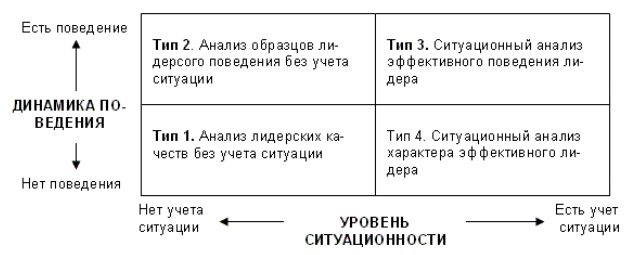
\includegraphics[width=\maxwidth{\textwidth}]{management-figures/leadership_methods}
	\caption{Подходы к изучению лидерства}
	\label{leadership_methods}
\end{figure}

\subsubsection{Управленческая решетка Блейка-Моутона}
Блэйк и Мутон исходили из того, что самым эффективным стилем руководства --- оптимальным стилем --- было поведение руководителя в позиции 9.9. 
По их мнению, такой руководитель сочетает в себе высокую степень внимания к своим подчиненным и такое же внимание к производительности.

\begin{figure}[h]
	\centering
	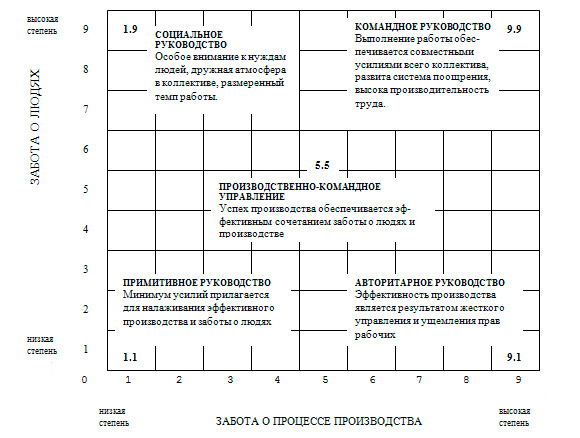
\includegraphics[width=\maxwidth{\textwidth}]{management-figures/leadership_lattice}
	\caption{Управленческая решетка Блейка-Моутона}
	\label{leadership_lattice}
\end{figure}

\subsection{Традиционные концепции лидерства}
\subsubsection{Теории Дугласа Макгрегора}
\begin{tabularx}{\textwidth}{X|X}
	\textbf{Теория <<X>>} & \textbf{Теория <<Y>>} \\ \hline
	В этой теории управление предполагает, что работники изначально ленивы и будут по возможности избегать работы. 
	Из-за этого работники должны быть под пристальным наблюдением, для чего разрабатываются комплексные системы контроля. 
	Необходима иерархическая структура с пониженной нормой управляемости на каждом уровне. 
	Согласно этой теории, работники проявляют мало амбиции без привлекательной программы поощрения и избегают ответственности, если это возможно.

	Менеджер по Теории X, как правило, считает, что всё должно заканчиваться возложением ответственности на кого-нибудь. 
	Он считает, что все предполагаемые работники ищут выгоды для себя. 
	Как правило, такие руководители полагают, что единственная цель заинтересованности сотрудников в работе --- это деньги. 
	В большинстве случаев они обвиняют в первую очередь человека, не ставя вопрос о том, что, может быть, винить надо систему, стратегию или отсутствие подготовки.
	&
	Управление предполагает, что работники могут быть амбициозными, иметь внутренние стимулы, стремиться взять на себя больше ответственности, осуществлять самоконтроль и самоуправление. 
	Считается, что сотрудники получают удовольствие от своих обязанностей, связанных как с умственным, так и физическим трудом. 
	Считается также, что работники испытывают желание проявлять творческое и прогрессивное мышление в производстве, если представляется возможность.

	Менеджер Теории Y считает, что при благоприятных условиях большинство людей хотят работать хорошо и, что у рабочей силы есть резерв неиспользуемых творческих способностей. 
	Они верят, что удовлетворение от хорошего выполнения своей работы само по себе является мощным стимулом. 
	Менеджер Теории Y постарается устранить препятствия, мешающие работникам полностью реализовать себя.
\end{tabularx}

\subsubsection{Теория К. Левина}
Она выделяет три стиля лидерства:
\begin{enumerate}
	\item \textbf{Авторитарный} \\
	Характеризуется жесткостью, требовательностью, единоначалием, превалированием властных функций, строгим контролем и дисциплиной, ориентацией на результат, игнорированием социально-психологических факторов.
	\item \textbf{Демократический} \\ 
	Опирается на коллегиальность, доверие, информирование подчиненных, инициативу, творчество, самодисциплину, сознательность, ответственность, поощрение, гласность, ориентацию не только на результаты, но и на способы их достижения.
	\item \textbf{Либеральный} \\ 
	Отличается низкой требовательностью, попустительством, отсутствием дисциплины и требовательности, пассивностью руководителя и потерей контроля над подчиненными, предоставлением им полной свободы действий.
\end{enumerate}

\subsubsection{Теория Лайкерта}
Согласно теории Лайкерта, различают четыре стиля руководства:
\begin{enumerate}
	\item \textbf{Эксплуататорско-авторитарный} \\
	Руководитель имеет четкие характеристики автократа, не доверяет подчиненным, редко привлекает их к принятию решений, а задачи формирует сам. 
	Основной стимул --- страх и угроза наказания, вознаграждения случайны, взаимодействие строится на взаимном недоверии. 
	Формальная и неформальная организация находятся в противоборстве.
	\item \textbf{Патерналистски-авторитарный} \\ 
	Руководитель благосклонно позволяет подчиненным принимать ограниченное участие в принятии решений. 
	Вознаграждение действительное, а наказание --- потенциальное, и то, и другое используется для мотивации работников. 
	Неформальная организация отчасти противостоит формальной структуре.
	\item \textbf{Консультативный} \\ 
	Руководитель принимает стратегические решения и, проявляя доверие, тактические решения делегирует подчиненным. 
	Ограниченное включение работников в процесс принятия решений используется для мотивации. 
	Неформальная организация не совпадает с формальной структурой лишь частично.
	\item \textbf{Демократический} \\ 
	Характеризуется полным доверием, основан на широком привлечении персонала к управлению организацией. 
	Процесс принятия решений рассредоточен по всем уровням, хотя и интегрирован. 
	Поток коммуникаций идет не только в вертикальных направлениях, но и по горизонтали. 
	Формальная и неформальная организации взаимодействуют конструктивно.
\end{enumerate}

\subsection{Концепции ситуационного лидерства}
Не существует одной лучшей стратегии руководства. 
В зависимости от готовности участников рабочей группы выполнять задания руководителя, он должен использовать одну из 4-х стратегий:
\begin{itemize}
	\item \textbf{Директивное управление} \\
	Руководитель говорит, указывает, направляет, устанавливает. 
	Жесткое назначение работ, строгий контроль сроков и результатов.
	\item \textbf{Объяснения} \\
	Лидер <<продает>>, объясняет, проясняет, убеждает. 
	Сочетание директивного и коллективного управления. 
	Объяснение своих решений.
	\item \textbf{Участие} \\
	Лидер участвует, поощряет, сотрудничает, проявляет преданность. 
	Приоритетное коллективное принятие решений, обмен идеями, поддержка инициативы подчиненных.
	\item \textbf{Делегирование} \\ 
	Лидер делегирует, наблюдает, обслуживает. 
	Не мешать --- пассивное управление сформировавшегося лидера.
\end{itemize}

\subsubsection{Континуум лидерского поведения Танненбаума-Шмидта}
% http://infomanagement.ru/lekciya/kontinuum_liderskogo_povedeniya
В соответствии с данной моделью лидер выбирает один из семи возможных образцов поведения в зависимости от силы воздействия на отношения лидерства трех факторов: самого лидера, его последователей и создавшейся ситуации. 
На рис.~\ref{leadership_tsh} показан весь спектр выборов между демократической и авторитарной альтернативами, соответственно ассоциируемыми с интересом к отношениям или к работе.

\begin{figure}[h]
	\centering
	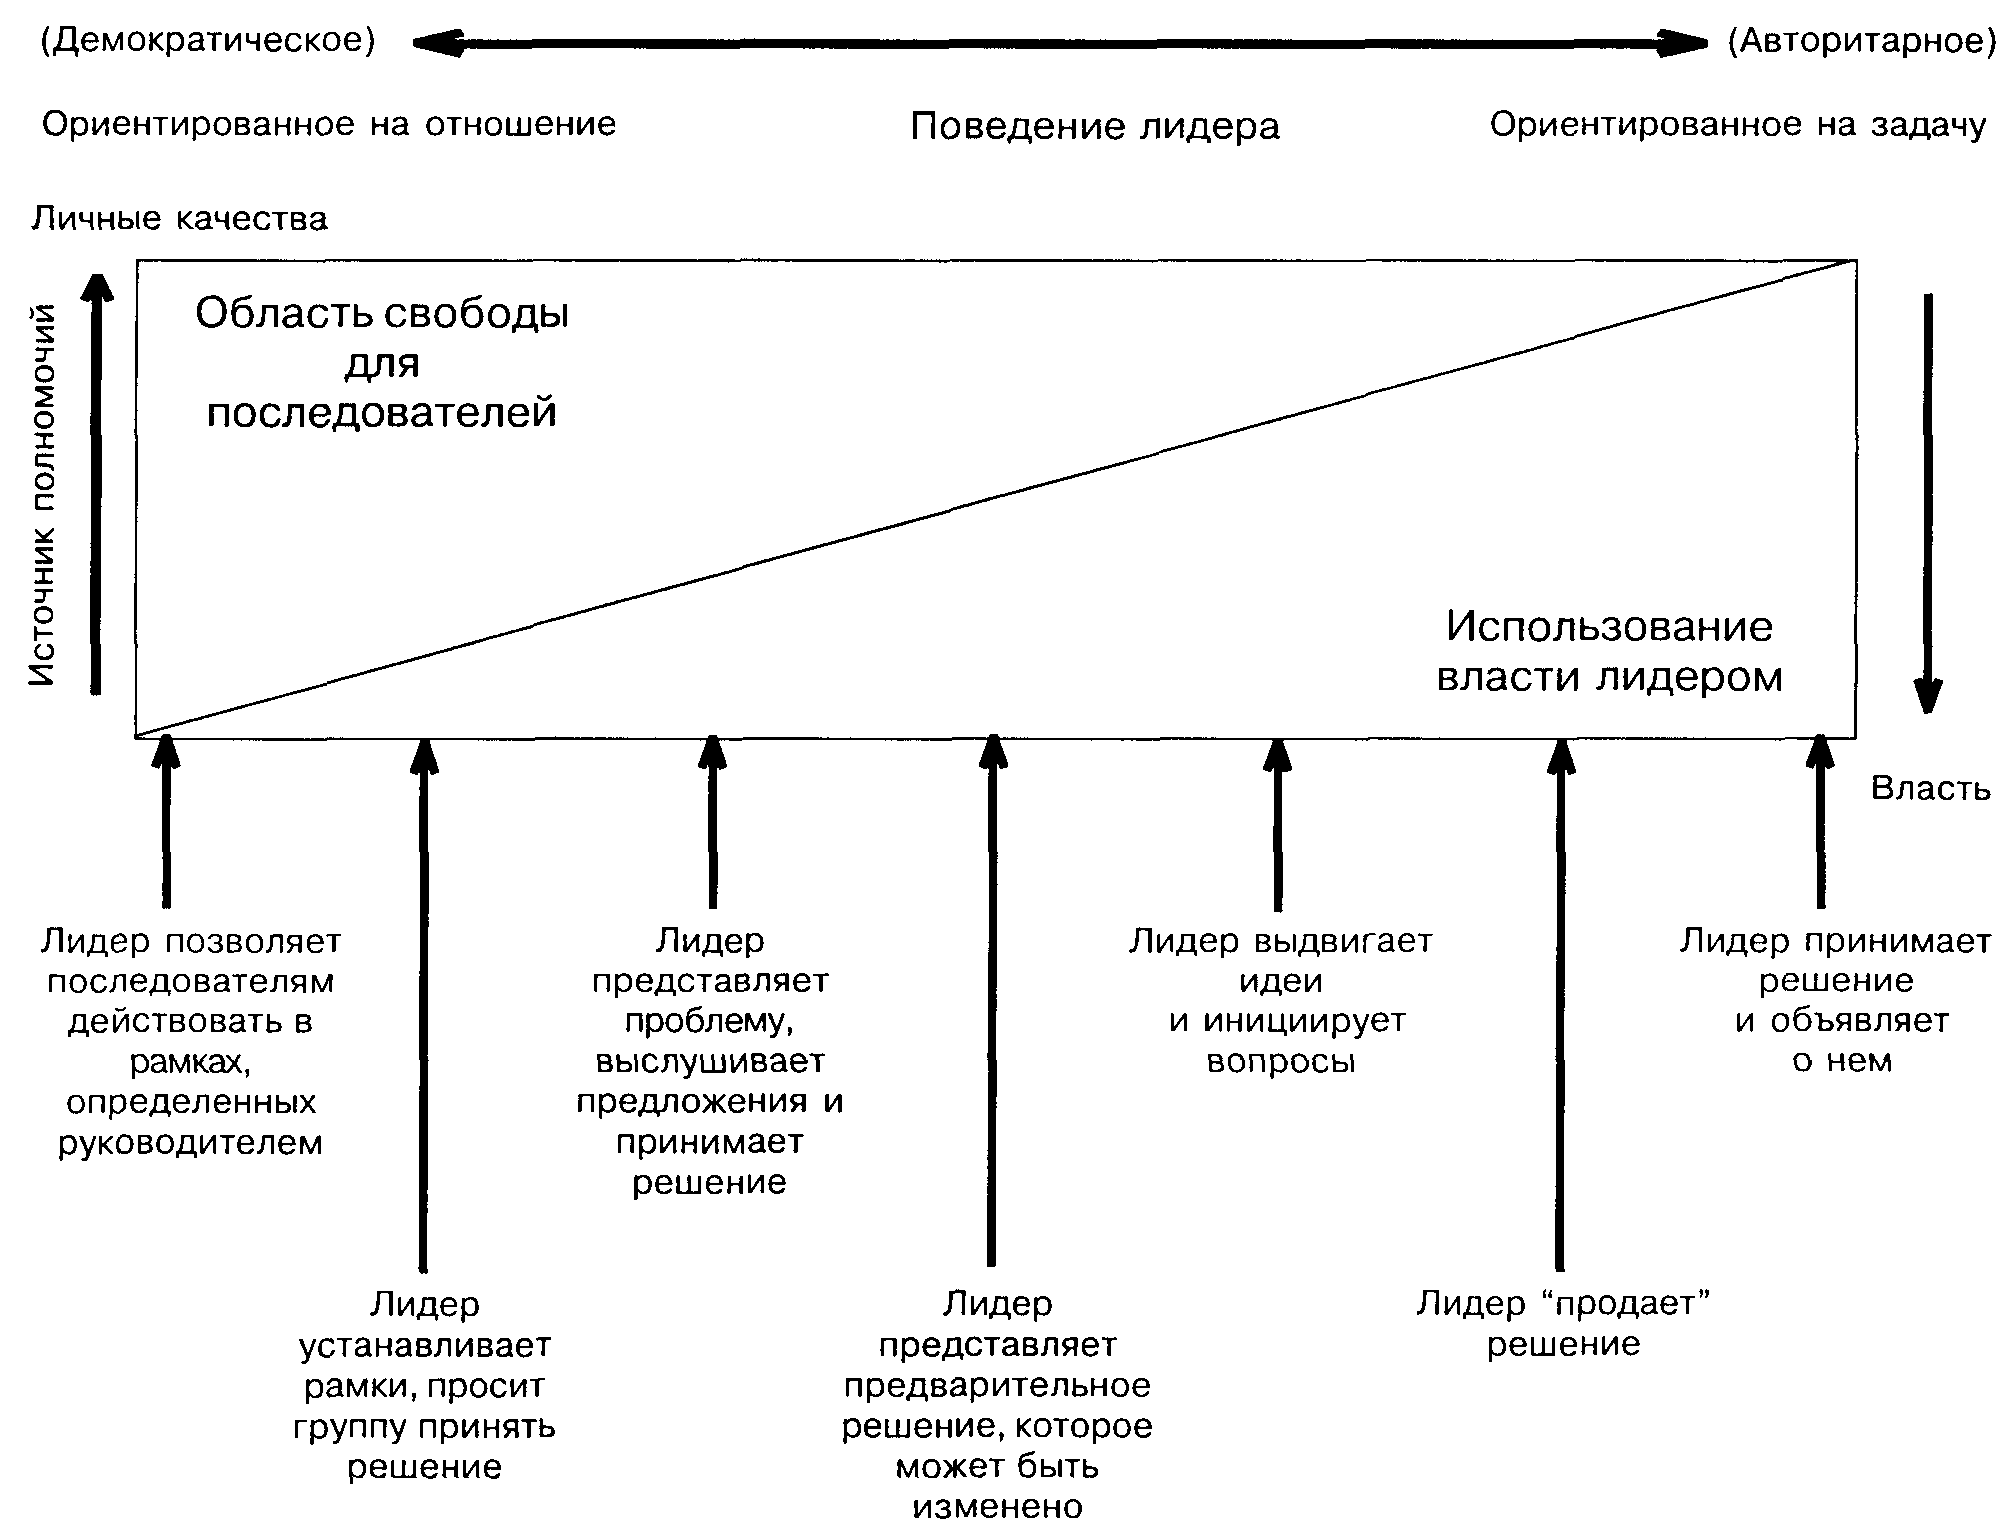
\includegraphics[width=\maxwidth{\textwidth}]{management-figures/leadership_tsh}
	\caption{Континуум лидерского поведения}
	\label{leadership_tsh}
\end{figure}

Различие между этими двумя крайними лидерскими стилями основано на предположениях лидера об источниках его власти и природе человека. 
Демократ полагает, что власть ему дается последователями, которых, он ведет, и что люди в своей основе обладают способностью к самоуправлению и творческой работе в условиях правильного мотивирования. 
Автократ считает, что власть дается его позицией в группе/организации и что люди внутренне ленивы и на них трудно полагаться. 
В первом случае имеется возможность, участия в управлении, во втором - цели, средства и политику определяет сам лидер.

\subsubsection{Модель лидерства <<путь-цель>> Хауза и Митчелла}
% http://infomanagement.ru/lekciya/model_liderstva
Рассматриваемая модель ситуационного лидерства получила своё развитие в 70-е годы. 
В своей основе она базируется на мотивационной теории ожидания. 
Исходной посылкой является предположение, что работники удовлетворены производительны тогда, когда имеется жесткая связь между и усилиями, и результатами работы, а также между результатом работы и вознаграждением. 
Отсюда модель получила свое название.
Существует прямая связь между уровнем лидерской эффективности уровнем мотивационной силы ожиданий, имеющихся последователей. 
Идеальным является вариант, когда вознаграждение полностью соответствует результату. 
Модель констатирует, что эффективный лидер --- это тот, кто помогает подчиненным идти путем ведущим к желаемой цели. 
При этом предлагаются различные варианты поведения лидера в зависимости от ситуации.

\begin{figure}[h]
	\centering
	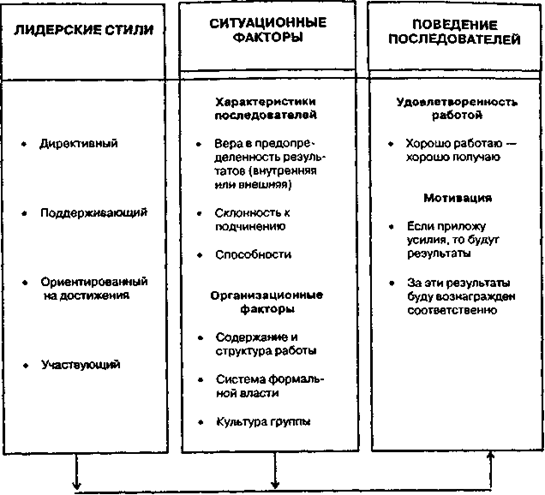
\includegraphics[width=\maxwidth{\textwidth}]{management-figures/leadership_wg}
	\caption{Модель лидерства <<путь-цель>> Хауза и Митчелла}
\end{figure}
\begin{itemize}
	\item \textbf{Директивное лидерство} \\
	Высокий уровень структурирования работы, объяснение подчиненным, что и как делать, а также что и когда от них ожидается.
	\item \textbf{Поддерживающее лидерство} \\ 
	Большое внимание нуждам работников и их благополучию, развитие дружественного рабочего климата и обращение с подчиненными как с равными.
	\item \textbf{Ориентированное на достижение} \\
	Установление напряженных, но притягательных целей, огромное внимание качеству во всем, уверенность в возможностях и способностях подчиненных достичь высокого уровня выполнения работы.
	\item \textbf{Участвующее лидерство} \\
	Совет с подчиненными и внимание к их предложениям и замечаниям в ходе принятия решений, привлечение подчиненных к участию в управлении.
\end{itemize}	

В отличие от концепции Фидлера, данная модель предполагает, что лидеры могут менять свое поведение и проявлять один или все из указанных стилей. 
Согласно модели, эффективная комбинация лидерских стилей зависит от ситуации.

Для анализа ситуации в модели предлагаются два типа ситуационных факторов: характеристики последователей и факторы организационной среды. 
Для описания характеристик последователей и выбора того или иного лидерского стиля используются следующие параметры:
\begin{enumerate}
	\item Вера в предопределенность происходящего от действий индивида. \\
	Выделяются два типа поведения подчиненных:
	\begin{itemize}
		\item люди внутренне уверены, что полученное вознаграждение определялось их усилиями;
		\item люди считают, что размер полученного вознаграждения контролировался внешними силами.
	\end{itemize}
	Первые предпочитают участвующий стиль лидерства, а вторые более удовлетворены директивным стилем.
	\item Склонность к подчинению. \\
	Данный параметр связан с наличием у индивида желания быть руководимым, внутренне соглашаться с влиянием других. 
	Те, кому присуще это, предпочитают в большей степени директивный стиль. 
	Другие стремятся активнее участвовать в управлении.
	\item Способности. \\ 
	Способности и имеющийся у последователей опыт определяют, насколько успешно они могут работать с лидером, ориентированным на достижение, или с лидером, привлекающим их к участию в управлении.
\end{enumerate}

В модели выделяются следующие факторы организационной среды, влияющие на выбор соответствующего лидерского стиля:
\begin{itemize}
	\item содержание и структура работы;
	\item формальная система власти в организации;
	\item групповая динамика и нормы.
\end{itemize}

Эти три фактора могут влиять на эффективность выбранного лидерского стиля в различных направлениях. 
Так, высоко структурированное задание не требует от лидера быть крайне директивным в управлении. 
Вместе с тем в организации с жесткой иерархией власти директивный лидер более эффективен, чем лидер, стремящийся привлечь подчиненных к участию в управлении. 
Забота лидера о нуждах подчиненных будет выглядеть несколько искусственно в группе с высокой степенью сплоченности. 
В целом в рамках того или иного лидерского стиля происходит взаимодействие между характеристиками последователей и организационными факторами, оказывающее влияние на восприятие мотивации последователями. 
В свою очередь восприятие, последователями, ситуации и уровень мотивации последователей определяют их удовлетворенность работой, уровень выполнения работы и признание лидера.

\subsubsection{Модель ситуационного лидерства Стинсона-Джонсона}
% http://infomanagement.ru/lekciya/model_situatsionnogo_liderstva_stinsona_jonsona
Данная модель исходит из того, что зависимость между поведением лидера и структурой работы задания является более сложной, чем это представлено в модели <<путь-цель>>. 
Модель констатирует, что хотя интерес к отношениям со стороны лидера более важен в случае, когда последователи выполняют высокоструктурированную работу, уровень интереса к работе при этом должен определяться лидером как в зависимости от характеристик последователей, так и характера самой работы, выполняемой ими.

Согласно модели, высокий интерес к работе со стороны лидера эффективен в следующих двух ситуациях:
\begin{itemize}
	\item работа высоко структурирована и последователи имеют сильную потребность в достижении и независимости. 
	При этом они обладают большими знаниями и опытом, чем им необходимо для выполнения работы;
	\item работа не структурирована, и последователи не испытывают потребности в достижении и независимости. 
	К тому же их знания и опыт ниже необходимого уровня.
\end{itemize}

Низкий интерес к работе эффективен для лидера в следующих двух ситуациях:
\begin{itemize}
	\item работа высоко структурирована и последователи испытывают потребности в достижении и независимости при наличии у них, достаточных знаний и опыта для выполнения данной работы;
	\item работа не структурирована, и последователи имеют сильную потребность в достижении и независимости при наличии у них больших знаний и опыта для выполнения данной работы. 
\end{itemize}

В табл.~\ref{tab:leadership_sj} показано поведение лидера в различных комбинациях структурированности работы и возможностей последователей. 
Модель убеждает ее пользователей, что характеристики последователей (их потребность в достижении и независимости, и их уровень знаний и опыта) являются критическими при выборе лидером эффективного стиля.

\begin{table}[h]
	\begin{tabularx}{\textwidth}{|X|X|X|}
		\hline
		& \multicolumn{2}{|c|}{Структурированность работы} \\ \hline
		& Низкая & Высокая \\ \hline 
		Возможности последователей --- высокие & Низкий интерес к отношениям и низкий интерес к работе & Высокий интерес к отношениям и высокий интерес к работе \\ \hline
		Возможности последователей --- низкие & Высокий интерес к работе и низкий интерес к отношениям & Высокий интерес к отношениям и низкий интерес к работе \\ \hline
	\end{tabularx}
	\caption{Выбор лидерского стиля в зависимости от ситуации}
	\label{tab:leadership_sj}
\end{table}

\subsubsection{Модель ситуационного лидерства Фидлера}
% http://infomanagement.ru/lekciya/model_situatsionnogo_liderstva_fidlera
Для измерения и определения лидерского стиля Фидлер предложил использовать разработанную им шкалу характеристик наименее предпочитаемого работника (НПР). 
В соответствии с этой шкалой. 
Респонденты должны, отмечать баллы по каждой из позиций шкалы, описать гипотетичесую личность, с которой они могли бы работать наименее успешно.

После того, как баллы подсчитаны по всем позициям шкалы, определяется стиль лидера.
Так, лидеры-респонденты, набравшие более высокие баллы, т.е. описавшие своего НПР очень позитивно, обладают стилем, ориентированным на отношения, а набравшие более низкие баллы имеют стиль, ориентированный на работу. 
Соответственно, эти два типа лидеров получили название лидер с высоким НПР и лидер с низким НПР. 
Согласно выводам Фидлера, лидерский стиль остается относительно постоянным и почти не меняется от ситуации к ситуации, так как в стиле отражены основы мотивации индивида: мотивированность на отношения и мотивированность на работу.

Степень контроля ситуации определяется в модели следующими тремя переменными:
\begin{enumerate}
	\item \textbf{Отношения <<лидер-последователь>>} \\
	Данная переменная отражает уровень лояльности, доверительности, поддержки и уважения, испытываемых и проявляемых последователем по отношению к лидеру.
	Речь идет о признании лидера последователями, что является наиболее важным условием обретения контроля над ситуацией. 
	Приняв лидера, последователи будут делать все возможное для достижения поставленных им целей.
	\item \textbf{Структурированность работы} \\
	Эта переменная отражает уровень структурированности решаемых группой проблем или выполняемых ею заданий и измеряется посредством следующих составляющих:
	\begin{itemize}
		\item ясность цели --- степень, с которой проблема или задание четко сформулированы или поставлены и знакомы исполнителям;
		\item множественность средств по достижению цели, степень возможности использования различных способов и путей. достижения цели, обоснованность решения --- степень <<правильности>> решения, подтверждаемая уровнем его принятия, его логикой или результатами.
	\end{itemize}
	Поскольку высокоструктурированная работа сама по себе содержит указания, что и как делать, то лидер получает в данной ситуации больший контроль над исполнителями.
	\item \textbf{Должностная власть} \\
	Рассматриваемая переменная отражает уровень формальной власти лидера, получаемой им на основе занимаемой в организации позиции, в частности, достаточность формальной власти для того, чтобы адекватно вознаграждать или, наказывать подчиненных, повышать их в должности или увольнять.
\end{enumerate}

На рис.~\ref{leadership_fd_var} приведена принципиальная схема взаимодействия лидерского стиля с ситуационными переменными.

\begin{figure}[h]
	\centering
	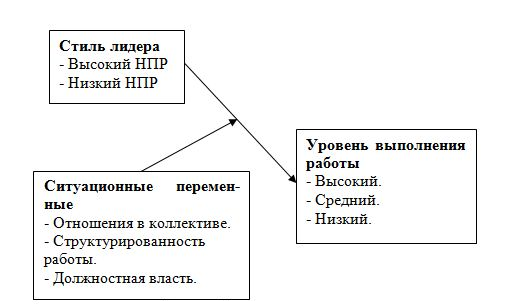
\includegraphics[width=\maxwidth{\textwidth}]{management-figures/leadership_fd_var}
	\caption{Переменные ситуационной модели Фидлера}
	\label{leadership_fd_var}
\end{figure}

Модель эффективного лидерства строится на том, что лидерство ситуационно. 
Три ситуационные переменные в сочетании с двумя лидерскими стилями дают восемь типов ситуаций (рис.~\ref{leadership_fd}), наглядно описывающих модель Фидлера.

\begin{figure}[h]
	\centering
	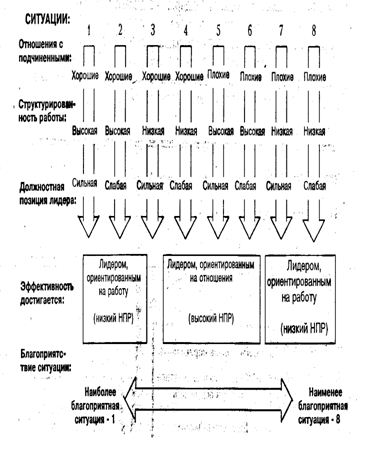
\includegraphics[width=\maxwidth{\textwidth}]{management-figures/leadership_fd}
	\caption{Типы ситуаций при использовании различных типов лидерства}
	\label{leadership_fd}
\end{figure}

\subsubsection{Модель ситуационного лидерства Херсея и Бланшарда}
% http://infomanagement.ru/lekciya/model_situatsionnogo_liderstva_herseya_i_blansharda
Данная модель равно как и другие концепции ситуационного лидерства, не предполагает поиска одного единственно верного пути для достижения эффективного лидерства. 
Вместо этого она делает упор на ситуационность лидерской эффективности. 
Одним из ключевых факторов ситуационности модель называет зрелость последователей, которая определяется степенью наличия у людей способностей и желания выполнять поставленную лидером задачу. 
Зрелость включает две составляющие: 
\begin{enumerate}
	\item Профессиональная --- это знания, умения и навыки, опыт, способности в целом. 
	Высокий уровень этой составляющей означает, что последователь не нуждается в директивах и указаниях.
	\item Психологическая зрелость --- соответствует желанию выполнять работу или мотивированности работника. 
	Высокий уровень этой составляющей у последователей не требует от лидера больших усилий по воодушевлению первых к работе, так как они уже внутренне замотивированы.
\end{enumerate}

Авторами модели были выделены четыре стадии зрелости последователей:
\begin{description}
	\item[М1] Люди не способны и не желают работать. 
	Они либо некомпетентны, либо не уверены в себе.
	\item[М2] Люди не способны, но желают работать. 
	У них есть мотивация, но нет навыков и умений.
	\item[М3] Люди способны, но не желают работать. 
	Их не привлекает то, что предлагает руководитель.
	\item[М4] Люди способны и желают делать то, что предлагает им лидер.
\end{description}

В зависимости от степени зрелости последователей лидер должен корректировать свои действия, относящиеся к установлению отношений с подчиненными и по структурированию самой работы. 
Таким образом,, модель строится на определении лидером соответствующих сложившейся ситуации уровней для поведения в области отношений \textit{(поддержка последователей)} и для поведения, относящегося к работе \textit{(директивность)}.

Поведение в области отношений связано с необходимостью для лидера больше прислушиваться к подчиненным, оказывать им поддержку, воодушевлять их и привлекать к участию в управлении. 
Поведение, относящееся к работе требует от лидера, проведения разъяснительной работы с последователями по поводу того, что и как они должны делать для того, чтобы выполнить поставленную перед ними задачу. 
Лидеры, ориентированные на такое поведение, структурируют, контролируют и внимательно следят за тем, как подчиненные работают. 
Сочетание этих двух типов лидерского поведения позволило в рамках данной модели выделить четыре основных лидерских стиля, каждый из которых наиболее соответствует определенной степени зрелости последователей:
\begin{enumerate}
	\item \textbf{Указывающий} стиль (S1) является лучшим в случае низкой зрелости последователей. 
	Лидер вынужден проявлять высокую директивность и тщательный присмотр за работниками, помогая таким образом людям, не способным и не желающим взять на себя ответственность по работе, устранить-неуверенность в том, что работа будет закончена.
	\item \textbf{Убеждающий} стиль (S2) является лучшим для использования в условиях умеренно низкой зрелости последователей, реализуя в равной мере директивность и поддержку тем, кто не способен, но желает работать. 
	Руководитель, использующий этот стиль, помогает им путем объяснения и вселяет в них уверенность в возможности выполнения задания.
	\item \textbf{Участвующий} стиль (S3) является лучшим при умеренно высокой зрелости последователей. 
	Способные к работе, но не желающие ее выполнять, подчиненные нуждаются в партнерстве со стороны лидера, чтобы быть более мотивированными на выполнение работы. 
	Предоставляя таким людям возможность участвовать в принятии решений на своем уровне, руководитель использует данный стиль, чтобы вызвать у последователей желание выполнять задание.
	\item \textbf{Делегирующий} стиль (S4) является лучшим для руководства высоко-зрелыми последователями. 
	Стиль характеризуется незначительной директивностью и поддержкой работников. 
	Это позволяет последователям, способным и желающим работать, взять на себя максимум ответственности за выполнение задания. 
	Данный лидерский стиль способствует развитию творческого подхода к работе.
\end{enumerate}

\begin{figure}[h]
	\centering
	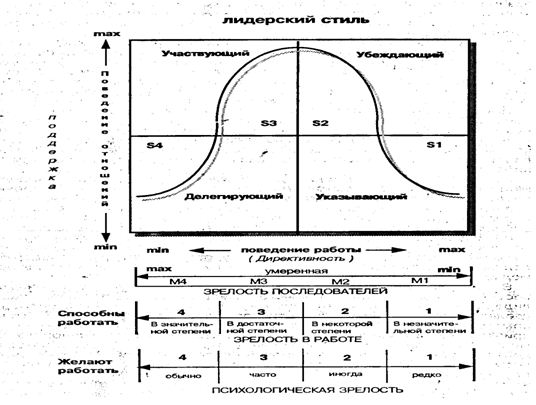
\includegraphics[width=\maxwidth{\textwidth}]{management-figures/leadership_hb}
	\caption{Модель ситуационного лидерства Херсея и Бланшарда}
\end{figure}

\subsubsection{Ситуационная модель принятия решений Врума-Йеттона-Яго}
% http://infomanagement.ru/lekciya/situatsionnaya_model
Одной из наиболее современных в объяснении ситуационного лидерства является модель, предложенная Виктором Врумом и Филиппом Йеттоном, которая позже была существенно дополнена с участием Артура Яго. 
Аналогично модели <<путь-цель>>, данная модель предлагает определять эффективный лидерский стиль в зависимости от ситуации. 
Предполагается также, что один и тот же лидер может использовать различные стили. 

Основным отличием модели является ее ориентированность только на один аспект лидерского поведения --- привлечение подчиненных к участию в принятии решений.
Соответственно лидеру предлагается концентрировать внимание на проблеме, которая должна быть решена, и на ситуации, в которой проблема возникла.
Подразумевается также, что ряд социальных процессов может оказать влияние на уровень участия подчиненных в решении проблем.

Главной идеей модели является то, что степень или уровень привлечения подчиненных к участию в принятии решения зависит от характеристик ситуации. 
В соответствии с моделью не существует одного единственно верного способа принятия решения, пригодного для всех ситуаций. 
После анализа и оценки каждого аспекта проблемы лидер определяет, какой стиль, с точки зрения участия подчиненных в принятии решения, ему лучше использовать.
В рассматриваемой модели эффективность решения $P_\textup{эфф}$ определяется на основе уравнения, показывающего, что она зависит от качества решения $P_\textup{кач}$ и уровня принимаемых подчиненными обязательств по выполнению решения $P_\textup{обяз}$, а также от степени срочности решения $P_\textup{время}$. 
Предпосылкой модели является представление, что отведенное ситуацией для решения время наряду с остальными двумя является, критическим фактором. 
Ситуация, в которой ограничение времени не играет роли, определяет этот показатель на нулевом уровне.
\[
P_\textup{эфф} = P_\textup{кач} + P_\textup{обяз} - P_\textup{время}
\]

Полная критериальная основа <<общей эффективности решения>> $O_\textup{эфф}$ предполагает учет в ней факторов <<стоимости>> и <<развития>>.
\[
O_\textup{эфф} = P_\textup{эфф} - \textup{стоимость} - \textup{развитие}
\]

В приведенной формуле показатель <<стоимость>> означает потерянное из-за решения время, которое в другом случае могло, принести больше пользы. 
Показатель <<развитие>> отражает тот выигрыш, который получен за пределами единолично принятого решения.

Последний разработанный вариант модели предлагает использование дерева решений для определения лидерского стиля, наиболее соответствующего сложившейся ситуации. 
При использовании модели менеджер как бы следует по ветвям этого дерева слева направо. 
Делая это он сталкивается с 10 проблемными ситуациями. 
Оценка ситуаций делается им по 8 аспектам проблемы с выбором по каждому из них ответа: высокий/высокая или низкий/низкая. 
Эти ответы выводят менеджера в конце концов на конкретную проблемную ситуацию и рекомендуемый для, нее стиль принятия решения (рис.~\ref{leadership_vyy_1}).

\begin{figure}[h]
	\centering
	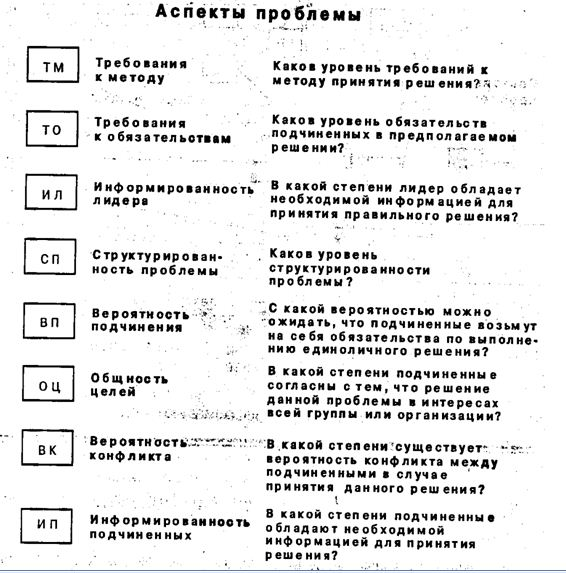
\includegraphics[width=\maxwidth{\textwidth}]{management-figures/leadership_vyy_1}
	\caption{Аспекты проблемы}
	\label{leadership_vyy_1}
\end{figure}

Для принятия решений в модели в зависимости от ситуации и степени привлечения подчиненных предлагается использовать пять стилей: 
\begin{description}
	\item[AI] Руководитель принимает решение сам, используя имеющуюся у него на данное время информацию.
	\item[АII] Руководитель получает необходимую информацию от своих подчиненных и затем сам принимает решение. 
	Работники привлекаются только на этапе сбора информации. 
	Выработку решения и его принятие осуществляет руководитель.
	\item[КI] Руководитель на индивидуальной основе делится соображениями по проблеме с имеющими к ней отношение подчиненными с целью получения от них идей и предложении, не собирая при этом их в группу. 
	Затем он сам принимает решение, которое может основываться на вкладе подчиненных, а может и нет.
	\item[КII] Руководитель делится соображениями по проблеме с подчиненными, собрав их вместе. 
	В ходе совещания он собирает их идеи и предложения. 
	Затем он принимает решение, которое может либо отражать, либо не отражать их вклад.
	\item[ГII] Руководитель делится соображениями по проблеме с оценивают альтернативы и пытаются достичь консенсуса относительно решения. 
	Роль, выполняемая при этом руководителем, больше похожа на роль председателя собрания, координирующего дискуссию. 
	Концентрирующего внимание на проблеме и делающего все для того, чтобы рассматривались наиболее важные аспекты проблемы. 
	Руководитель не пытается влиять на группу с тем, чтобы она приняла его решение, и проявляет готовность принять и выполнить любое решение, получившее поддержку всей группы. 
\end{description}

Одной из отличительных особенностей модели является то, что в целом она делает больший упор на изучение ситуации, чем на изучение личности лидера.
Действительно, может быть, имеет больше смысла говорить об автократической ситуации и ситуации участия, чем об автократическом лидере или участвующем лидере.

\begin{figure}[h]
	\centering
	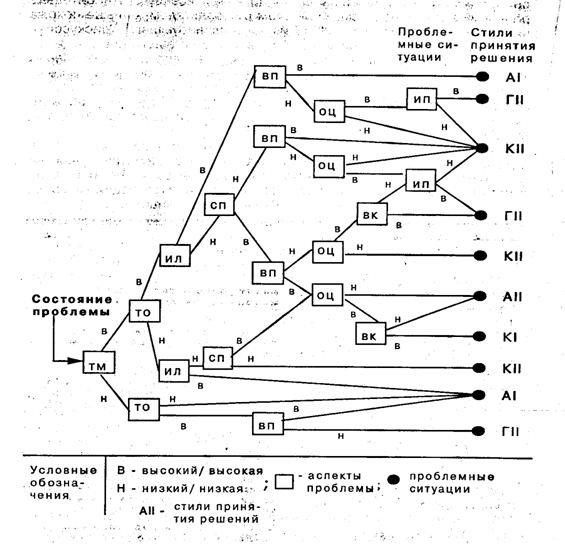
\includegraphics[width=\maxwidth{\textwidth}]{management-figures/leadership_vyy_2}
	\caption{Дерево решений Врума-Яго}
	\label{leadership_vyy_2}
\end{figure}

\subsection{Новое в теориях лидерства}
\subsubsection{Атрибутивное лидерство}
Концепция атрибутивного лидерства основана на причинно-следственных связях между тем, что произошло и тем, что люди считают причиной произошедшего. 
Такую связь объясняет теория атрубуции. 
Атрибутивный подход исходит из того, что выбор лидера, в равной мере, как и поведение последователей, обусловлены реакцией лидера на поведение последних.
Наблюдая за работой сотрудников, лидер получает информацию о том, как она выполняется. 
В зависимости от этого он делает выводы о поведении каждого работника и корректирует стиль своего поведения таким образом, чтобы адекватно реагировать на действия подчиненного. 

Атрибутивное лидерство пытается ответить на вопрос, почему люди ведут себя так, а не иначе. 
Определение лидером причин поведения последователя базируется на трех признаках: личность, сама работа, организационное окружение или обстоятельства.

В поиске причин лидер пытается получить три вида информации о поведении последователей:
\begin{enumerate}
	\item \textbf{Степень отличия задания} \\
	Это связано с желанием лидера понять связь между поведением и работой с той точки зрения, насколько определенное поведение может быть вызвано отличительными особенностями задания. 
	\item \textbf{Последовательность поведения работника} \\ 
	Лидера интересует то, насколько подчиненный последователен в проявлении данного поведения или как часто это поведение у него повторяется.
	\item \textbf{Степень уникальности поведения} \\
	Лидер учитывает, насколько другие подчиненные ведут себя таким же образом, т.е. является ли данное поведение уникальным, характерным для одного подчиненного или наблюдается у всей группы. 
\end{enumerate}

Технология развития данного лидерства сосредоточена на двух задачах:
\begin{itemize}
	\item создание (поддержание) харизматического образа какого-либо человека;
	\item формирование его отношений с последователями. 
\end{itemize}

\subsubsection{Харизматическое лидерство}
Харизма --- одаренность человека, его исключительность. 
Харизматическим считается лидер, который способен оказывать глубокое воздействие на последователей в силу своих личностных качеств. 
В целом харизматическому лидеру приписывают уверенность в себе, стремление к власти, убежденность в совей правоте, нестандартное видение решения проблемы, умение обосновать его перед последователями и побудить их к действию, неординарное поведение при реализации своего видения. 
Присущая такому человеку жажда деятельности передается другим людям, и они искренне верят в прирожденную способность к лидерству. 

Значение харизматического лидерства для бизнеса возрастает по мере необходимости проведения в организации радикальных изменений. 
В стабильной ситуации оно не всегда эффективно. 

\subsubsection{Преобразующее лидерство} 
Это лидерство эффективно в ситуациях изменений, динамического развития, реинжиниринга бизнес-процессов. 

Лидер-реформатор мотивирует последователей путем:
\begin{itemize}
	\item повышения уровня их сознательности в восприятии поставленной цели;
	\item предоставления им возможности соотношения своих личных интересов с общей целью;
	\item создания атмосферы доверительности и убеждения последователей в необходимости саморазвития. 
\end{itemize}

Лидер-реформатор --- это новатор, стратег-преобразователь, а не спаситель, его цель не изменить мир, а адаптироваться в нем через развитие персонала, организационное развитие. 
Модель преобразующего лидерства предполагает наличие у лидера последователей определенного поведения, которое наиболее подходит для творческого решения проблемы в кризисной ситуации.

\subsection{Природа конфликта и стресса}
Конфликт --- это отсутствие согласия между двумя и более сторонами, которыми могут быть как конкретные лица, группы, так и организации в целом, причем это несогласие между сторонами приводит к тому, что сознательное поведение одной из сторон вступает в противоречие с интересами другой стороны.

Причины: распределение ресурсов, взаимозависимость задач, различие в целях, различие в представлениях и ценностях, различие в манерах поведения и жизненном опыте и неудовлетворительных коммуникациях.

Типы конфликтов:
\begin{itemize}
	\item внутриличностный;
	\item межличностный;
	\item между личностью и группой;
	\item внешний.
\end{itemize}

Позитивные функции конфликта.
\begin{itemize}
	\item разрядка напряженности между сторонами;
	\item сплочение коллектива перед внешним врагом. Широко известно, что дружить легче против кого-то;
	\item несомненно, внешний враг может помочь усилению консолидации членов группы;
	\item получение новой информации об оппоненте и окружающей социальной среде;
	\item большая расположенность к сотрудничеству в будущем;
	\item снятие синдрома покорности у подчиненных.
\end{itemize}

Негативные функции конфликта.
\begin{itemize}
	\item большие эмоциональные и материальные затраты на участие в конфликте;
	\item рост неудовлетворенности, плохое моральное состояние;
	\item снижение производительности труда, рост текучести кадров;
	\item представление о второй стороне как о враге;
	\item уменьшение сотрудничества после завершения конфликта;
	\item сложное восстановление деловых отношений (<<шлейф>> конфликта);
	\item усиление тенденции к авторитарному руководству.
\end{itemize}

\subsection{Управление конфликтной ситуацией}
% http://www.nnre.ru/delovaja_literatura/menedzhment_konspekt_lekcii/p12.php
Управление конфликтом --- это целенаправленное воздействие на устранение причин конфликта или на коррекцию поведения участников. 
Методы управления и разрешения конфликтов делятся на три группы: внутриличностные, структурные и межличностные.

Внутриличностные методы воздействуют на отдельную личность и состоят в правильной организации своего собственного поведения, в умении высказывать свою точку зрения, не вызывая защитной реакции со стороны оппонента.

Структурные методы изменяют структуру заданий работникам или структуру организации. 
К структурным методам разрешения конфликтов относятся следующие:
\begin{enumerate}
	\item Разъяснение требований к работе. 
	\item Использование координационных и интеграционных механизмов, которые улучшают согласованность между подразделениями и отдельными людьми.
	\item Постановка общеорганизационных целей.
	\item Использование системы вознаграждений для поощрения поведения, направленного на избежание негативных последствий конфликтов.
\end{enumerate}

Методы разрешения межличностных конфликтов через сотрудничество:
\begin{enumerate}
	\item Определите проблему в категориях целей, а не решений.
	\item После того, как проблема определена, определите решения, которые приемлемы для обеих сторон.
	\item Сосредоточьте внимание на проблеме, а не на личных качествах другой стороны.
	\item Создайте атмосферу доверия, увеличив взаимное влияние и обмен информацией.
	\item Во время общения создайте положительное отношение друг к другу, проявляя симпатию и выслушивая мнения другой стороны, а также сводя к минимуму проявления гнева и угроз.
\end{enumerate}

\subsection{Управление изменениями}
Управление изменениями --- это структурный подход к переводу индивидов, команд и организаций из текущего состояния в желаемое будущее состояние. 
Целью этого организационного процесса является расширение прав и возможностей сотрудников принять и поддержать изменения в их текущем бизнес-окружении. 
В управлении проектами, управление изменениями рассматривается как процесс управления проектом, в котором формально представлены и одобрены изменения проекта.

В управлении изменениями используются различные подходы для анализа, подготовки и проведения изменений:
\begin{enumerate}
	\item Индивидуальные изменения.
	\item Командные изменения.
	\item Организационные изменения.
\end{enumerate}

Использование типовых шагов для проведения изменений подробно рассмотрено в работах Коттера, таких как:
\begin{enumerate}
	\item Преодоление состояния удовлетворенности текущей ситуацией.
	\item Формирование команды для проведения изменения.
	\item Определение видения желаемого будущего и стратегии перехода.
	\item Широкое информирование о проводимых изменениях.
	\item Устранение препятствий и барьеров, мешающих проведению изменений.
	\item Достижение быстрых первых успехов.
	\item Поддержание процесса изменений с целью недопущения отката назад.
	\item Закрепление проведенных изменений в корпоративной культуре.
\end{enumerate}

Управление изменениями оперирует такими понятиями, как лидерство, эффективность коммуникаций и принятие потребности в изменениях для разработки точных стратегий перехода, для того чтобы преодолеть неизбежное сопротивление переменам.

\subsection{Сущность, функции и элементы маркетинга}
Маркетинг --- это комплексная система организации производства и сбыта, ориентированная на возможное более полное удовлетворение быстро меняющихся и все более разнообразных потребностей потребителей посредством рынка и получение на этой основе устойчивой прибыли и конкурентных преимуществ.

Выделяют 3 (три) подхода к определению сущности маркетинга:
\begin{itemize}
	\item как самостоятельный вид производственной деятельности;
	\item как функция управления;
	\item как современное видение философии бизнеса.
\end{itemize}

Концепция маркетинга --- это философия управления, которая способствует получению товара производителями прибыли посредством удовлетворения потребностей потребителей.

% http://www.grandars.ru/student/marketing/funkcii-marketinga.html
Главные функции маркетинга:
\begin{itemize}
	\item аналитическая функция;
	\item продуктово-производственная функция;
	\item сбытовая функция (функция продаж);
	\item функция управления и контроля.
\end{itemize}

Комплекс маркетинга --- совокупность управляемых элементов маркетинговой деятельности организации, манипулируя которыми она старается наилучшим образом удовлетворить потребности целевых рынков.
% https://ru.wikipedia.org/wiki/%D0%A2%D0%B5%D0%BE%D1%80%D0%B8%D1%8F_4P
Теория 4P \textit{(маркетинг-микс)} — маркетинговая теория, основанная на четырёх основных <<координатах>> маркетингового планирования:
\begin{description}
	\item[Product] Товар или услуга, ассортимент, качество, свойства товара, дизайн и эргономика.
	\item[Price] Цена, наценки, скидки.
	\item[Promotion] Продвижение, реклама, пиар, стимулирование сбыта.
	\item[Place] Месторасположения торговой точки, каналы распределения, персонал продавца.
\end{description}

\subsection{Задачи, виды и структура маркетинговых исследований}
Маркетинговое исследование --- это систематический поиск, сбор, анализ и представление данных и сведений, относящихся к конкретной рыночной ситуации, с которой пришлось столкнуться предприятию. 
Маркетинговое исследование можно также определить как систематический сбор, учет и анализ данных по маркетингу и маркетинговым проблемам в целях совершенствования качества процедур принятия решений и контроля в маркетинговой среде. 
Имеется целый ряд аналогичных и иных определений маркетинговых исследований.

Основные цели маркетингового исследования:
\begin{itemize}
	\item уменьшить неопределенность и минимизировать риск в процессе принятия управленческих решений;
	\item следить за процессом реализации маркетинговых задач.
\end{itemize}

Глобальные цели маркетингового исследования --- это информационное обеспечение маркетинга, то есть сбор необходимой информации и аналитическое обеспечение, заключающееся в использовании математических моделей для анализа данных и получения с их помощью прогнозов и возможности принятия оптимальных решений.

% http://works.doklad.ru/view/hARiKdLaWJM.html
Задачи маркетинговых исследований могут быть самыми разнообразными и диктоваться потребностями разработки стратегии маркетинга, формирование ценовой, товарной, коммуникационной, сбытовой политики и другими аспектами управления маркетингом на предприятии. 
Наиболее типичные решаемые задачи маркетинговых исследований:
\begin{itemize}
	\item изучение характеристик рынка;
	\item замеры потенциальных возможностей рынка;
	\item анализ распределения долей рынка между фирмами;
	\item анализ сбыта;
	\item изучение тенденций деловой активности;
	\item изучение товаров конкурентов;
	\item краткосрочное прогнозирование;
	\item изучение реакции на новый товар и его потенциала;
	\item долгосрочное прогнозирование;
	\item изучение политики цен.
\end{itemize}

\begin{figure}[h]
	\centering
	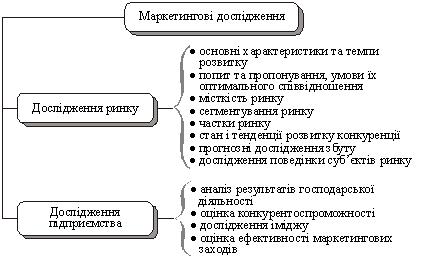
\includegraphics[width=\maxwidth{\textwidth}]{management-figures/marketing_structure}
	\caption{Структура маркетинговых исследований}
\end{figure}

Типы маркетинговых исследований:
\begin{enumerate}
	\item \textbf{Разведочные} или поисковые, предшествующие разработке программы основного исследования. 
	Предпринимаются для сбора предварительной информации, освещающие проблемы, позволяет выдвинуть гипотезы.
	\item \textbf{Описательные} \textit{(дескриптивные)}. 
	Имеющие целью констатацию реальных фактов, событий, показателей, полученных в результате сбора информации. 
	\item \textbf{Экспериментальные}. 
	Проводится с целью проверки выдвинутой гипотезы.
	\item \textbf{Аналитические}. 
	Проводимое для выявления и моделирования связи и деятельности фирмы с факторами окружающей среды. 
\end{enumerate}

\subsection{Маркетинговое сегментирование рынка}
Сегментирование рынка --- это процесс разделения рынка на отдельные части --- сегменты, отличающиеся друг от друга разными возможностями сбыта.

Сегмент рынка --- это особым образом выделенная часть рынка, группы потребителей или предприятий, обладающих определенными общими признаками. 
Может быть осуществлено по множеству критериев --- мерилам оценки обоснованности выбора сегмента рынка. 
Принцип сегментирования --- показатель выделения данного сегмента рынка. 

\begin{figure}[h]
	% http://powerbranding.ru/segmentirovanie/osnovy/
	\centering
	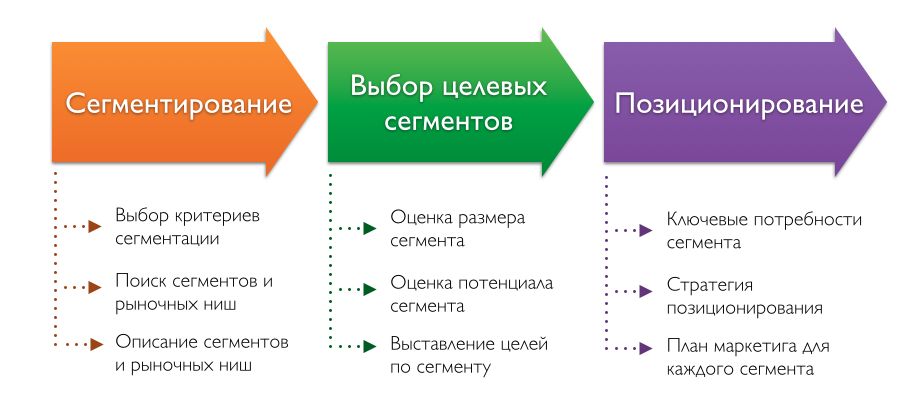
\includegraphics[width=\maxwidth{\textwidth}]{management-figures/marketing_segmentation_process}
	\caption{Схема сегментации рынка}
\end{figure}

Могут быть использованы следующие критерии:
\begin{enumerate}
	\item Различия между потребителями позволяющее объединить их в один сегмент.
	\item Сходство, формирующие устойчивость.
	\item Наличие показателей, позволяющих измерить характеристики и требования потребителей, определить емкость рынка.
	\item Возможность выстоять в конкурентной борьбе.
	\item Достаточность объема продаж.
	\item Доступность сегмента для предприятия.
\end{enumerate}

Существует три варианта охвата рынка:
\begin{itemize}
	\item недифференцированный маркетинг;
	\item дифференцированный маркетинг;
	\item концентрированный маркетинг.
\end{itemize}

На выбор стратегии охвата рынка влияют ресурсы фирмы, степень однородности продукции, этапы жизненного цикла товара, степень однородности рынка.

Обобщенные критерии правильного определения сегмента:
\begin{itemize}
\item доступность;
\item измеримость;
\item значимость по размерам, динамике спроса и своему совокупному потенциалу;
\item заметные отличия от других составных частей рынка;
\item относительная устойчивость сходства спроса со стороны потребителей.
\end{itemize}

\subsection{Цель и суть товарной политики}
Товарная политика --- это совокупность решений, касающихся формирования эффективной рыночно-ориентированной производственной программы предприятия.

Товарная политика ­­--- область целенаправленных действий по отдельным предложенным для использования товарам и услугам (вид, количество, свойство и т.д.), а также по совокупности отдельных продуктов (ширина, глубина, структура ассортимента).

Цель товарной политики --- добиться сбалансированного товарного ассортимента и конкурентоспособности каждого отдельного продукта, а так же:
\begin{itemize}
	\item обеспечение прибыли;
	\item увеличение товарооборота;
	\item увеличение доли рынка;
	\item снижение расходов на производство и маркетинг;
	\item повышение имиджа;
	\item рассеивание риска.
\end{itemize}

Задачи товарной политики --- принятие решений в области предлагаемых предприятием товаров, касающихся самих продуктов, их присутствия на рынке, а также связанных с этим решений по производственной программе.

\subsection{Использование средств стимулирования сбыта}
% http://www.aup.ru/books/m99/7_9.htm
Стимулирование сбыта --- это совокупность приемов, применяемых на протяжении всего жизненного цикла товара в отношении трех участников рынка (потребителя, оптового торговца, продавца), для краткосрочного увеличения объема сбыта, а также для увеличения числа новых покупателей.

Стимулирование сбыта имеет многоцелевую направленность: потребитель, продавец, торговый посредник.

Выбор средств стимулирования зависит от поставленных целей. 
Все средства можно объединить в три большие группы:
\begin{itemize}
	\item предложение цены (продажа по сниженным ценам, льготные купоны, талоны, дающие право на скидку);
	\item предложение в натуральной форме (премии, образцы товара);
	\item активное предложение (конкурсы покупателей, игры, лотереи).
\end{itemize}

Процесс выбора комплекса продвижения товара включает этапы:
\begin{enumerate}
	\item Определение цели продвижения. 	
	\begin{enumerate}
		\item Информирование потребителей.
		\item Стимулирование сбыта.
		\item Формирование благоприятного имиджа.
		\item Влияние на привычки потребителей.
		\item Поддержание деловых отношений, взаимопонимание с деловыми партнерами и т.д.
	\end{enumerate}
	\item Оценивание факторов, влияющих на комплекс продвижения.		
	\begin{enumerate}
		\item Цели фирмы.
		\item Стратегия.
		\item Целевая аудитория.
		\item Тип товара.
		\item Этап жизненного цикла.
		\item Объем рынка.
		\item Стоимость.
	\end{enumerate}
	\item Разработка стратегии продвижения.	
	\begin{enumerate}
		\item Интенсификация рекламы.
		\item Новая рекламная компания.
	\end{enumerate}
	\item Составление и распределение бюджета распределения.	
	\begin{enumerate}
		\item <<Снизу-вверх>>. Общая сумма затрат на комплекс продвижения.
		\item <<Сверху-вниз>>. Составляем статьи отдельно для рекламы, персональной продажи, а потом считаем общую сумму.
	\end{enumerate}
	\item Методы составления бюджета.	
	\item Оценивание комплекса продвижения.	
\end{enumerate}

\subsection{Ценовая политика в маркетинговой деятельности. Методы расчета и установления цены}
Цена --- денежное выражение стоимости товара, предназначенное для непрямого измерения общественно-необходимых затрат рабочего времени на производство товара. Количество денежных единиц, которые должен заплатить покупатель продавцу за весь товар или его единицу.

Ценовая политика --- это установление определенных цен и способов маневрирование ими в зависимости от положения на рынке, которые позволяют овладеть долю рынка, получить расчетную прибыль, а также решить другие стратегические и оперативные задачи.

На цену влияют внешние факторы (политическая стабильность страны, экономика, гос. регулирование цены, состояние рынка) и внутренний (стратегия и тактика фирмы, специфика жизненного цикла товара, особенности производства и характеристики системы продвижения товаров на рынке).

Алгоритм определение цены:
\begin{enumerate}
	\item Определение целей. 	
	\item Определение и анализ спроса. 	
	\item Анализ издержек производства. 	
	\item Анализ цен товаров конкурентов. 	
	\item Методы ценообразования. 	
	\item Выбор ценовой стратегии. 	
	\item Адаптация цен. 	
\end{enumerate}

Методы ценообразования:
\begin{itemize}
	\item ориентированный на затратах;
	\item ориентированная на спрос;
	\item ориентируемые на конкурентов.
\end{itemize}

\end{document}